% !TeX root = proyecto.tex

%=========================================================
\chapter{Modelo dinámico}	
\label{cap:modDinamico}

\cdtInstrucciones{Presente la solución indicando el si esta se compone de varios sistemas, los subsistemas del sistema y si aplica, los módulos de los subsistemas.}

	Este capítulo describe en modelo dinámico del sistema. en el se detallan todos los escenarios de ejecución del sistema. La figura~\ref{fig:casosDeUso} muestra el diagrama general del sistema y sus subsistemas, y la figura~\ref{fig:casosDeUsoDetalle} muestra todos los casos de uso del sistema. En este documento solo detallamos los casos de uso del subsistema de gestión de cursos.
	
\begin{figure}[htbp]
	\begin{center}
		\fbox{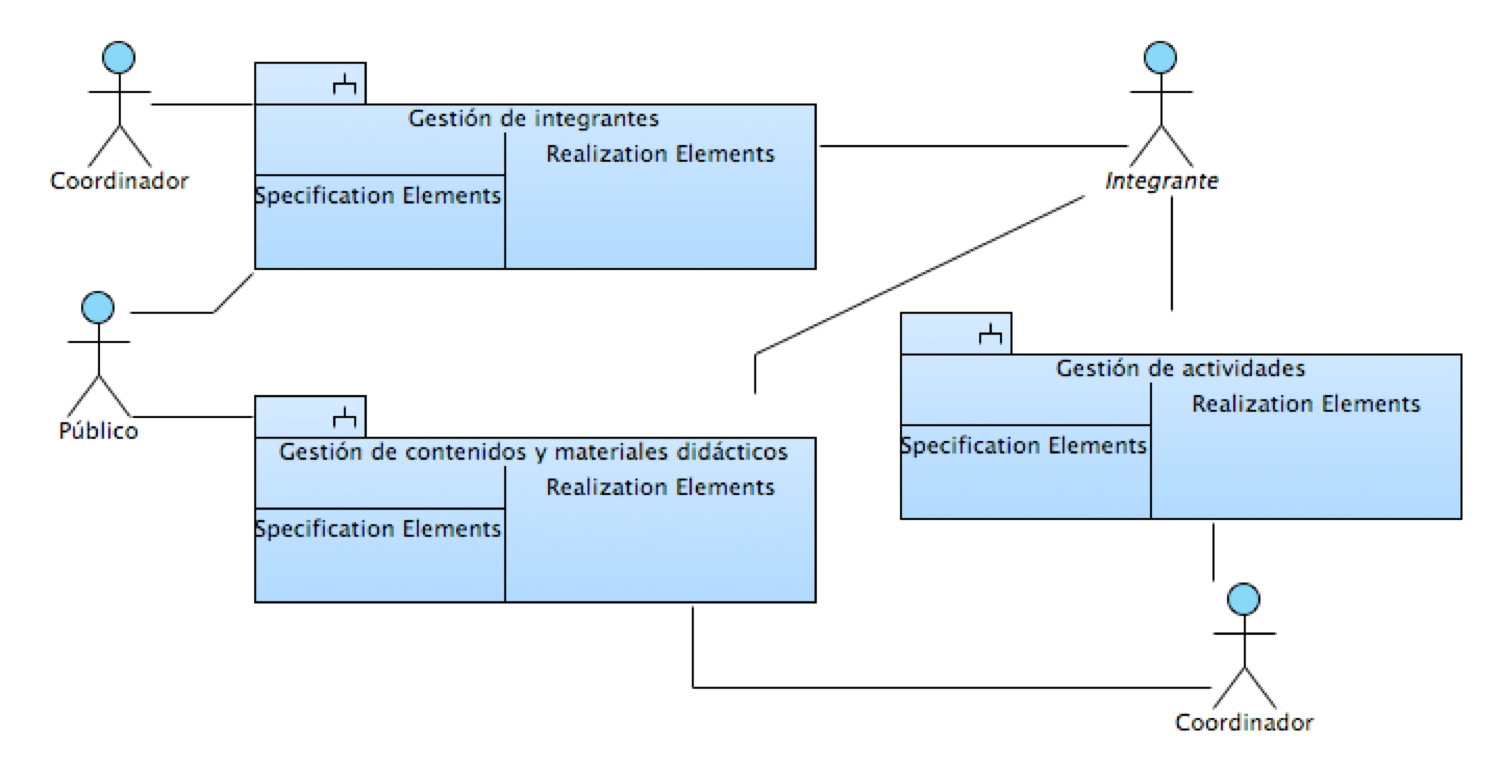
\includegraphics[width=.8\textwidth]{images/casosDeUso}}
		\caption{Diagrama de casos de uso del sistema.}
		\label{fig:casosDeUso}
	\end{center}
\end{figure}

\begin{figure}[htbp]
	\begin{center}
		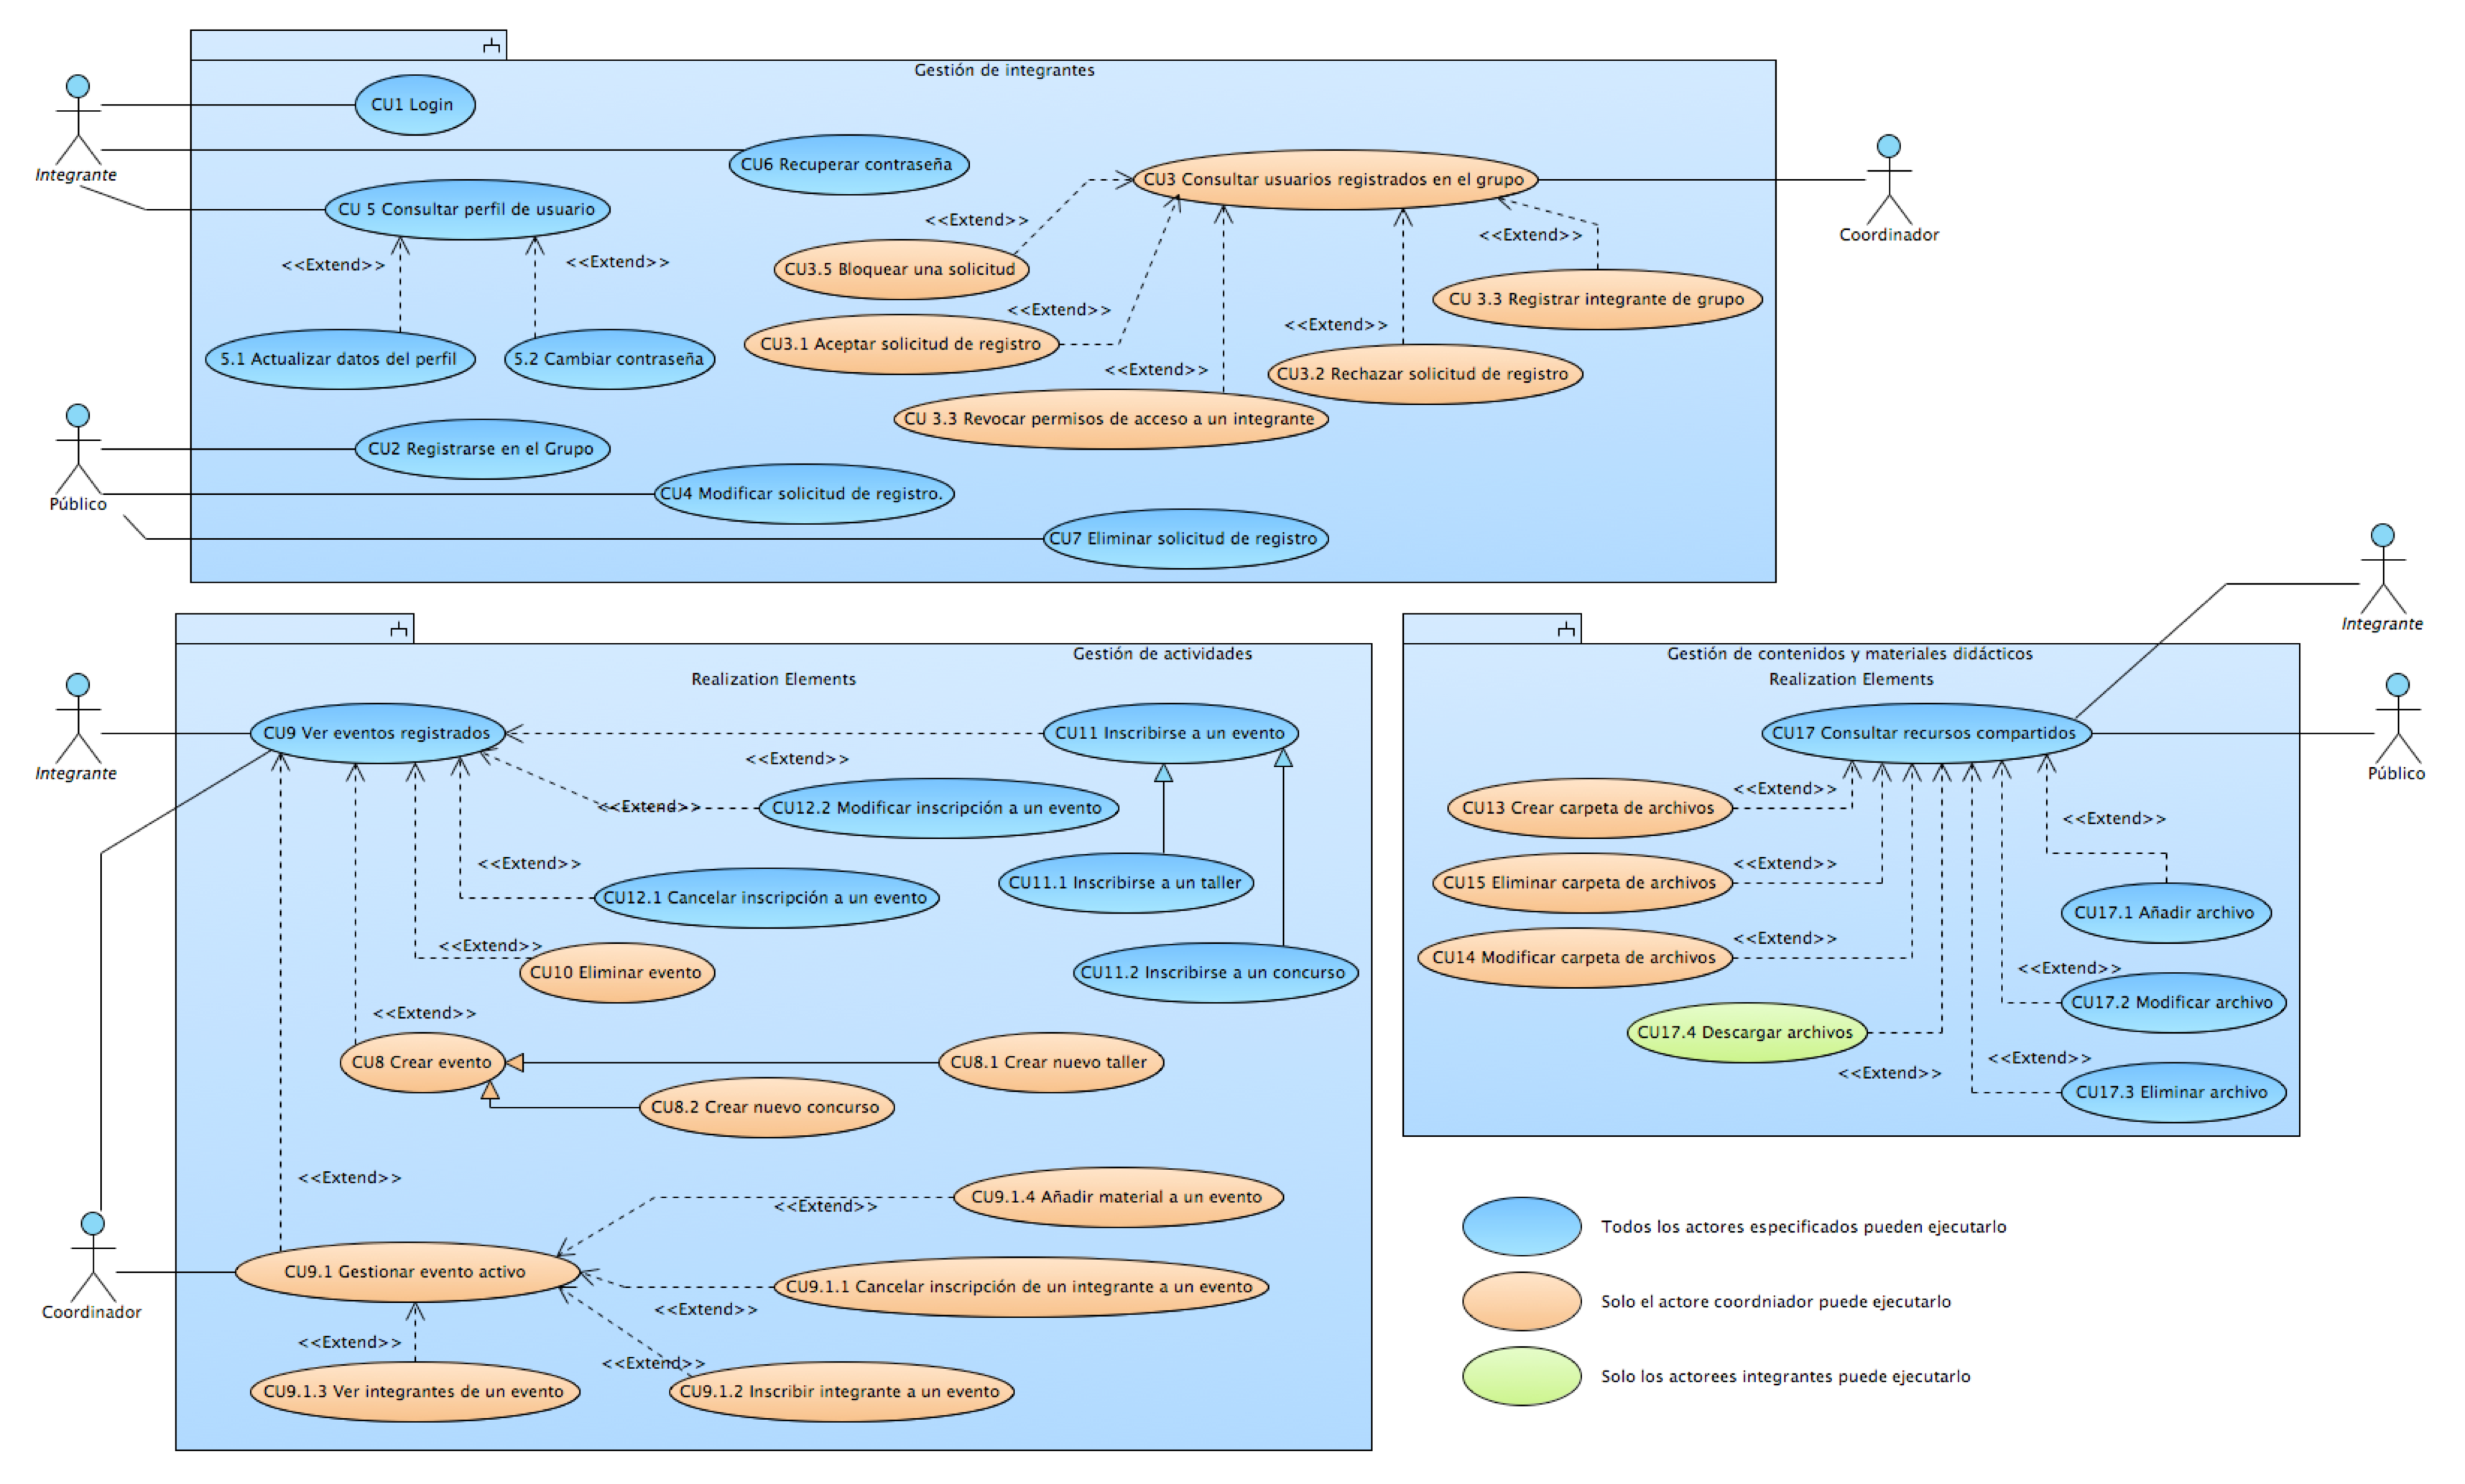
\includegraphics[angle=90, width=.7\textwidth]{images/casosDeUsoDetalle}
		\caption{Diagrama detallado del sistema.}
		\label{fig:casosDeUsoDetalle}
	\end{center}
\end{figure}

%---------------------------------------------------------
\section{Descripción de casos de uso}



A continuación se detallan los casos de uso.

%---------------------------------------------------------
% CASOS DE USO

%!TEX root = ../proyecto.tex

% Plantilla para caso de uso sencillo con ejemplos de comandos e intrucciones.
%-------------------------------------- COMIENZA descripción del caso de uso.

%\begin{UseCase}[archivo de imágen]{UCX}{Nombre del Caso de uso}{
%--------------------------------------
\begin{UseCase}{CU1}{Registrar Cliente}{
	Cuando un cliente quiere reservar en el hotel, se debe dar de alta en el sistema con sus datos personales, una vez registrado podrá ingresar al sistema.
}
	\UCitem{Versión}{\color{Gray}
		0.2	% Ponga un número de versión, 
	}\UCitem{Autor}{\color{Gray}
		Ruiz Evaristo Marco Antonio. % Analista responsable de especificar el CU
	}\UCitem{Supervisa}{\color{Gray}
		Hernández Jiménez Erick Yael. % Analista responsable de verificar que está correcto.
	% TODO: Dar de alta al actor Usuario
	}\UCitem{Actor}{
		\hyperlink{Cliente}{Cliente} % No olvide dar de alta el actor.
	}\UCitem{Propósito}{\begin{Titemize}%Indique los fines, objetivos, propósitos o valores agregados del Caso de uso.
		\Titem Permitir al cliente realizar reservaciones y registrar mascotas.
		\Titem Garantizar la privacidad de los datos del cliente y soportar la responsabilidad de los clientes en el sistema.
	\end{Titemize}
	}\UCitem{Entradas}{\begin{Titemize}
		% TODO: Dar de alta las entidades que se listan.
		\Titem \hyperlink{Cliente.nombre}{Nombre(s)} del cliente % El identificador no acepta acentos, espacios ni eñes.
		\Titem \hyperlink{Cliente.primerApellido}{Primer apellido} del cliente % Liste todos los datos de entrada
		\Titem \hyperlink{Cliente.segundoApellido}{Segundo apellido} del cliente. 
		\Titem \hyperlink{Cliente.CURP}{CURP } del cliente
		\Titem \hyperlink{Cliente.telefono}{Numero telefonico} del cliente.
		\Titem \hyperlink{Cliente.correo}{Correo electónico} del cliente
		\Titem \hyperlink{Cliente.direccion}{Ubicación origen} coordenadas latitud y longitud.
		\Titem \hyperlink{Cliente.Atributo}{Contraseña} con confirmación.
		\end{Titemize}
	}\UCitem{Origen}{\begin{Titemize}
		\Titem Se introducen desde el teclado y mouse.
		\Titem Ubicacion origen. La selecciona el usuario en el mapa % Indique por que medio se introducen los datos, 
	\end{Titemize}
	}\UCitem{Salidas}{\begin{Titemize}
		% TODO: Dar de alta las entidades que se listan.
		\Titem Mensajes de error. %Agregar errores explícitamente
		
	\end{Titemize}
	}\UCitem{Destino}{\begin{Titemize}
%		\Titem Se muestra en la pantalla \IUref{IU01}{}.. % Indique por que medio se muestran los datos, 
%		\Titem otros.          % Si es ḿas de uno indique que datos corresponden en cada medio de entrada.
		\Titem Se muestra en la pantalla \IUref{IU1}{Registrar cliente}.
	\end{Titemize}
	}\UCitem{Precondiciones}{\begin{Titemize}
		\Titem No debe haber otro cliente registrado con el mismo CURP ni correo electrónico.
	\end{Titemize}
	}\UCitem{Postcondiciones}{\begin{Titemize}
		\Titem Habrá un nuevo cliente registrado en el sistema.
		\Titem El cliente podrá registrar mascotas.
		\Titem El cliente podrá realizar reservaciones.
		\Titem El cliente podrá iniciar sesión.
		\Titem Se mostrara la pantalla \IUref{IU5}{Home cliente}
	\end{Titemize}
	}\UCitem{Errores}{\begin{Titemize}
		% Escriba todos los errores que puedan ocurrir en el sistema, para cada error recuerde:
		% Punerle un identificador
		% Describir la condición o escenario que detona el error
		% Describa la forma en que debe reaccionar el sitema: si la reaccion corresponde a varios pasos use mejor una trayectoria alternativa.
		% Relacione el error con la trayectoria principal.
		\Titem {\bf \hypertarget{CU1.E1}{E1}}: Cuando el cliente no haya llenado algun campo obligatorio, el sistema muestra el mensaje \MSGref{MSG-001}{Campo obligatorio} y regresa al paso \ref{UC1.paso3}.
			\Titem {\bf \hypertarget{CU1.E2}{E2}}: Cuando el CURP del cliente ya este registrado en el sistema, el sistema muestra el mensaje \MSGref{MSG-005}{CURP ya existente} y regresa al paso \ref{UC1.paso3}.
			\Titem {\bf \hypertarget{CU1.E3}{E3}}: Cuando el correo electronico del cliente ya este registrado en el sistema, el sistema muestra el mensaje \MSGref{MSG-006}{Correo electrónico ya existente} y regresa al paso \ref{UC1.paso3}
			\Titem {\bf \hypertarget{CU1.E4}{E4}}: Cuando el cliente ingrese un tipo de dato diferente al solicitado, el sistema muestra el mensaje \MSGref{MSG-007}{Dato no válido} y regresa al paso \ref{UC1.paso3}
			
	\end{Titemize}
	}\UCitem{Tipo}{
		% Especifique el tipo de caso de us, puede ser: "Caso de uso primario" o 
		% "Viene de \\hyperref{CUY}{CUY nombre del CU}" cuando se desprende desde otro caso de uso mediante un extends.
		Caso de uso primario
	}\UCitem{Observaciones}{
		% Indique las observaciones al caso de uso, las cuales pueden ser:
		%
		 Ninguna
		% - Dudas sobre el procedimiento o la especificación.
		% - Issues detectados
		% - Suposiciones realizadas.
		% - Cualquier otra especificacion que considere pertinente que no pudo colocarse en los demás atributos del Caso de uso
		% - Aclaraciones.
		% - Notas para el usuario o desarrollador.
		% - Pendientes (TODO's) en caso de no usar los comentarios.
	}
\end{UseCase}

%--------------------------------------
\begin{UCtrayectoria}
	% Cada paso debe inicair con un Verbo en infinitivo, siempre especificando el objetivo del paso mas la accion en concreto.
	% \UCpaso[\UCactor] se refiere al actor y \UCpaso se refiere al sistema.
	% A continuación viene ejemplos de pasos:
	% En el siguiente paso: "Ingresa al sistema" es el objetivo del paso y "escribiendo la URL de la aplicación" es la acción en concreto.
	\UCpaso[] \label{UC1.paso1}El cliente indica al sistema que desea registrarse presionando el botón \IUbutton{Registrar cliente} de la pantalla \IUref{IU3}{Pantalla de inicio}.
    \UCpaso[] \label{UC1.paso2}El sistema solicita los datos personales del cliente mediante la pantalla \IUref{IU1}{Registrar Cliente}.
    \UCpaso[] \label{UC1.paso3} El cliente proporciona sus datos personales.
    \UCpaso[] \label{UC1.paso4} El cliente solicita el registro mediante el botón \IUbutton{Registrar} de la pantalla \IUref{IU2}{Registrar Cliente}.
    \UCpaso[] El sistema verifica que todos los campos obligatorios se hayan llenado \ErrorRef{CU1}{E1}{Campo obligatorio}.
    \UCpaso[] El sistema verifica que los datos introducidos tengan un formato válido en los campos correspondientes \ErrorRef{CU1}{E4}{Dato no válido}.
    \UCpaso[] \label{UC1.paso5} El sistema verifica que no haya un cliente ya registrado con el mismo CURP \ErrorRef{CU1}{E2}{CURP ya existente}.
    \UCpaso[] \label{UC1.paso6} El sistema verifica que no haya un cliente ya registrado con el mismo correo electrónico \ErrorRef{CU1}{E3}{Correo electrónico ya existente}.
    \UCpaso[] \label{UC1.paso7} El sistema muestra la pantalla \IUref{IU5}{Home cliente} con el mensaje \MSGref{MSG-003}{No hay reservaciones}.
\end{UCtrayectoria}


%--------------------------------------
% Las trayectorias alternativas se identifican con Letras: A, B, C, etc.


%--------------------------------------
% Puntos de extensión

% Comente la siguiente sección en caso de que no hayan puntos de extensión o relaciones de tipo extends.
%\subsection{Puntos de extensión}
%\UCExtenssionPoint{
	% Cuando se dá la extensión del Caso de uso:
%	El usuario no recuerda cual es su contraseña o sospecha que su usuario está bloqueado.
%}{
	% Durante la región (en que pasos se puede dar la extensión):
%	Del paso \ref{CUX.etiqueta} al paso \ref{CUX.etiqueta}.
%}{
	% Casos de uso a los que extiende:
%	\UCref{CUZ}{Nombre del caso de uso}.
%}
		
		
		
%-------------------------------------- TERMINA descripción del caso de uso.
%!TEX root = ../proyecto.tex

% Plantilla para caso de uso sencillo con ejemplos de comandos e intrucciones.
%-------------------------------------- COMIENZA descripción del caso de uso.

%\begin{UseCase}[archivo de imágen]{UCX}{Nombre del Caso de uso}{
%--------------------------------------
\begin{UseCase}{CU2}{Registrar Reservación}{
		Cuando un cliente quiere realizar una reservación en hotel, debe registrar sus datos de reservación, una vez registrados se creara la reservación y se mostraran los detalles de la misma.
	}
	\UCitem{Versión}{\color{Gray}
		0.3	% Ponga un número de versión, 
	}\UCitem{Autor}{\color{Gray}
		Hernández Jiménez Erick Yael. % Analista responsable de especificar el CU
	}\UCitem{Supervisa}{\color{Gray}
		Ruiz Evaristo Marco Antonio. % Analista responsable de verificar que está correcto.
		% TODO: Dar de alta al actor Usuario
	}\UCitem{Actor}{
		\hyperlink{Cliente}{Cliente}% No olvide dar de alta el actor.
	}\UCitem{Propósito}{\begin{Titemize}%Indique los fines, objetivos, propósitos o valores agregados del Caso de uso.
		\Titem Proporcionar a los clientes un medio conveniente para realizar reservaciones para sus mascotas, permitiendo planificar sus necesidades de cuidado con anticipación.
		\Titem Gestionar la disponibilidad de las reservaciones, evitando conflictos y asegurando que los recursos estén bien distribuidos.
		\Titem Asegurar que todos los datos relevantes se ingresen de manera correcta y completa para el uso efectivo de los servicios.
		\Titem Ofrecer un medio para enviar recordatorios al cliente sobre las reservas próximas, reduciendo así el riesgo de cancelaciones tardías o ausencias.
		\end{Titemize}
	}\UCitem{Entradas}{\begin{Titemize}
			\Titem \hyperlink{SUCURSAL.NOMBRE_SUCURSAL}{Sucursal}.
			\Titem \hyperlink{DISPONIBILIDAD.CHECK-IN}{Check-in}
			\Titem \hyperlink{DISPONIBILIDAD.CHECK-OUT}{Check-out}.
			\Titem \hyperlink{ESPECIE.NOMBRE_ESPECIE}{Especies} de las mascotas a hospedar.
			\Titem \hyperlink{RAZA.NOMBRE_RAZA}{Razas} de las mascotas a hospedar.
			\Titem Número de mascotas de la misma raza que el cliente desea hospedar.
			\Titem \hyperlink{TAMANO.TAMANO}{Tamaños} de las mascotas a hospedar.
			\Titem \hyperlink{TIPO_CUARTO.NOMBRE_CUARTO}{Nombre de los cuartos} que desea reservar el cliente.
			\Titem \hyperlink{TIPO_SERVICIO.NOMBRE_SERVICIO}{Nombre de los servicios} que desea adquirir para la mascota el cliente.
		\end{Titemize}
	}\UCitem{Origen}{\begin{Titemize}
			\Titem \hyperlink{SUCURSAL.NOMBRE_SUCURSAL}{Sucursal}: Menú desplegable en la pantalla \IUref{IU6}{Búsqueda de hospedajes}.
			\Titem \hyperlink{DISPONIBILIDAD.CHECK-IN}{Check-in}: Selector de fechas en la pantalla \IUref{IU6}{Búsqueda de hospedajes}.
			\Titem \hyperlink{DISPONIBILIDAD.CHECK-OUT}{check-out}: Selector de fechas en la pantalla \IUref{IU6}{Búsqueda de hospedajes}.
			\Titem \hyperlink{ESPECIE.NOMBRE_ESPECIE}{Especies}: Menú desplegable en la pantalla \IUref{IU6}{Búsqueda de hospedajes}.
			\Titem \hyperlink{RAZA.NOMBRE_RAZA}{Razas}: Menú desplegable en la pantalla \IUref{IU6}{Búsqueda de hospedajes}.
			\Titem \hyperlink{TAMANO.TAMANO}{Tamaños}: Menú desplegable en la pantalla \IUref{IU6}{Búsqueda de hospedajes}.
			\Titem \hyperlink{TIPO_CUARTO.NOMBRE_CUARTO}{Nombre de los cuartos}: Botones de selección en la pantalla \IUref{IU7}{Catálogo de habitaciones}.
			\Titem \hyperlink{TIPO_SERVICIO.NOMBRE_SERVICIO}{Nombre de servicios}: Menú desplegable en la pantalla \IUref{IU9}{Servicios adicionales}.
		\end{Titemize}
	}\UCitem{Salidas}{\begin{Titemize}
			\Titem \hyperlink{SUCURSAL.NOMBRE_SUCURSAL}{Sucursal}.
			\Titem \hyperlink{DISPONIBILIDAD.CHECK-IN}{Check-in}.
			\Titem \hyperlink{DISPONIBILIDAD.CHECK-OUT}{Check-out}.
			\Titem \hyperlink{ESPECIE.NOMBRE_ESPECIE}{Especies} de las mascotas a hospedar.
			\Titem \hyperlink{RAZA.NOMBRE_RAZA}{Razas} de las mascotas a hospedar.
			\Titem \hyperlink{TAMANO.TAMANO}{Tamaños} de las mascotas a hospedar.
			\Titem \hyperlink{TIPO_CUARTO.NOMBRE_CUARTO}{Nombre de los cuartos} que desea reservar el cliente.
			\Titem \hyperlink{TIPO_CUARTO.PRECIO_CUARTO}{Precio del los cuartos} que desea reservar el cliente.
			\Titem \hyperlink{SUCURSAL.CALLE_DIRECCION}{Calle} de la sucursal en la que reserva el cliente.
			\Titem \hyperlink{SUCURSAL.NUMERO_DIRECCION}{Número de calle} de la sucursal en la que reserva el cliente.
			\Titem \hyperlink{SUCURSAL.NOMBRE_COLONIA_DIRECCION}{Colonia} de la sucursal en la que reserva el cliente.
			\Titem \hyperlink{SUCURSAL.NOMBRE_MUNICIPIO_DIRECCION}{Municipio} de la sucursal en la que reserva el cliente.
			\Titem \hyperlink{SUCURSAL.CODIGO_POSTAL_DIRECCION}{Código postal} de la sucursal en la que reserva el cliente.
			\Titem \hyperlink{SUCURSAL.ENTIDAD_DIRECCION}{Entidad} de la sucursal en la que reserva el cliente.
			\Titem \hyperlink{TIPO_SERVICIO.NOMBRE_SERVICIO}{Nombre de los servicios} que desea adquirir para la mascota el cliente.
			\Titem \hyperlink{TIPO_SERVICIO.COSTO_BASE}{Costo base de los servicios} que desea adquirir para la mascota el cliente.
			\Titem \hyperlink{TIPO_SERVICIO.COSTO_EXTRA}{Costo extra de los servicios} que desea adquirir para la mascota el cliente en caso de presentarse la necesidad de servicios emergentes.
			\Titem \hyperlink{CORTE_RESERVACION.SUMA_PRECIO_CUARTOS}{Total de los cuartos} que contrata el cliente.
			\Titem \hyperlink{CORTE_RESERVACION.SUMA_PRECIO_CITAS_SERVICIOS}{Total de los servicios} que contrata el cliente.
			\Titem \hyperlink{CORTE_RESERVACION.SUMA_TOTAL_RESERVACION}{Suma total por el hospedaje} que contrata el cliente.
		\end{Titemize}
	}\UCitem{Destino}{\begin{Titemize}
			\Titem \hyperlink{SUCURSAL.NOMBRE_SUCURSAL}{Sucursal}: En la pantalla  \IUref{IU7}{Catálogo de habitaciones} y \IUref{IU8}{Vista general del cuarto}.
			\Titem \hyperlink{DISPONIBILIDAD.CHECK-IN}{Check-in}: En la pantalla \IUref{IU7}{Catálogo de habitaciones} y \IUref{IU8}{Vista general del cuarto}.
			\Titem \hyperlink{DISPONIBILIDAD.CHECK-OUT}{check-out}: En la pantalla \IUref{IU7}{Catálogo de habitaciones} y \IUref{IU8}{Vista general del cuarto}.
			\Titem \hyperlink{ESPECIE.NOMBRE_ESPECIE}{Especies}: En la pantalla \IUref{IU7}{Catálogo de habitaciones} y \IUref{IU8}{Vista general del cuarto}.
			\Titem \hyperlink{RAZA.NOMBRE_RAZA}{Razas}: En la pantalla \IUref{IU7}{Catálogo de habitaciones} y \IUref{IU8}{Vista general del cuarto}.
			\Titem \hyperlink{TAMANO.TAMANO}{Tamaños}: En la pantalla \IUref{IU7}{Catálogo de habitaciones} y \IUref{IU8}{Vista general del cuarto}.
			\Titem \hyperlink{TIPO_CUARTO.NOMBRE_CUARTO}{Nombre de los cuartos}: En la pantalla \IUref{IU7}{Catálogo de habitaciones} y \IUref{IU8}{Vista general del cuarto}.
			\Titem \hyperlink{TIPO_CUARTO.PRECIO_CUARTO}{Precio de los cuartos}: En la pantalla \IUref{IU7}{Catálogo de habitaciones} y \IUref{IU8}{Vista general del cuarto}.
			\Titem \hyperlink{SUCURSAL.CALLE_DIRECCION}{Calle}: En un mapa en la pantalla \IUref{IU8}{Vista general del cuarto}.
			\Titem \hyperlink{SUCURSAL.NUMERO_DIRECCION}{Número de calle}: En un mapa en la pantalla \IUref{IU8}{Vista general del cuarto}.
			\Titem \hyperlink{SUCURSAL.NOMBRE_COLONIA_DIRECCION}{Colonia}: En un mapa en la pantalla \IUref{IU8}{Vista general del cuarto}.
			\Titem \hyperlink{SUCURSAL.NOMBRE_MUNICIPIO_DIRECCION}{Municipio}: En un mapa en la pantalla \IUref{IU8}{Vista general del cuarto}.
			\Titem \hyperlink{SUCURSAL.CODIGO_POSTAL_DIRECCION}{Código postal}: En un mapa en la pantalla \IUref{IU8}{Vista general del cuarto}.
			\Titem \hyperlink{SUCURSAL.ENTIDAD_DIRECCION}{Entidad}: En un mapa en la pantalla \IUref{IU8}{Vista general del cuarto}.
			\Titem \hyperlink{TIPO_SERVICIO.NOMBRE_SERVICIO}{Nombre de los servicios}: En la pantalla \IUref{IU9}{Servicios adicionales}.
			\Titem \hyperlink{TIPO_SERVICIO.COSTO_BASE}{Costo base de los servicios}: En la pantalla \IUref{IU9}{Servicios adicionales}.
			\Titem \hyperlink{TIPO_SERVICIO.COSTO_EXTRA}{Costo extra de los servicios}: En la pantalla \IUref{IU9}{Servicios adicionales}.
			\Titem \hyperlink{CORTE_RESERVACION.SUMA_PRECIO_CUARTOS}{Total de los cuartos}: En la pantalla \IUref{IU9}{Servicios adicionales} y en la pantalla \IUref{IU11}{Resumen del hospedaje}.
			\Titem \hyperlink{CORTE_RESERVACION.SUMA_PRECIO_CITAS_SERVICIOS}{Total de los servicios}: En la pantalla \IUref{IU9}{Servicios adicionales} y en la pantalla \IUref{IU11}{Resumen del hospedaje}.
			\Titem \hyperlink{CORTE_RESERVACION.SUMA_TOTAL_RESERVACION}{Suma total por el hospedaje}: En la pantalla \IUref{IU9}{Servicios adicionales} y en la pantalla \IUref{IU11}{Resumen del hospedaje}.
		\end{Titemize}
	}\UCitem{Precondiciones}{\begin{Titemize}
			% Incluya Precondiciones lógicas, de negocio e incluso las que debe atender el usuario. 
			\Titem Debe haber al menos un cuarto en al menos una sucursal.
			\Titem El cliente debe acceder al sistema por el caso de uso \UCref{CUX}{Iniciar Sesion} o \UCref{CU1}{Registrar Cliente}.
			\Titem Debe haber disponibilidad de habitaciones en las fechas deseadas.
		\end{Titemize}
	}\UCitem{Postcondiciones}{\begin{Titemize}
			\Titem Habrá una nueva reservación registrada para este cliente en el sistema.
			\Titem El calendario de disponibilidad se ha actualizado para reflejar las fechas reservadas.
			\Titem El cliente ha recibido una confirmación de la reservación a traves de la pantalla \IUref{IU5}{Home Cliente} y de un correo electrónico.
			\Titem Se habilitará el botón \IUbutton{Mascotas} en la pantalla \IUref{IU5}{Home Cliente}
			\Titem Todas las mascotas que el cliente haya asociado a la reservación serán accesibles para el cliente en la pantalla \IUref{IUX}{Consultar mascotas propias}.
		\end{Titemize}
	}\UCitem{Errores}{\begin{Titemize}
			\Titem {\bf \hypertarget{CU2.E1}{E1}}: Cuando el cliente no haya iniciado sesión en el sistema, se le indica que es \MSGref{MSG-013}{Necesario iniciar sesión} y dirige al cliente al caso de uso \IUref{CU1}.
			\Titem {\bf \hypertarget{CU2.E2}{E2}}: Cuando el cliente no haya ingresado los datos mínimos necesarios para la operación, se le muestra el mensaje  \MSGref{MSG-001}{Campo obligatorio} y regresa al paso anterior.
			\Titem {\bf \hypertarget{CU2.E3}{E3}}: Cuando el cliente ingrese un tipo de dato diferente al solicitado, el sistema muestra el mensaje \MSGref{MSG-007}{Dato no válido} y regresa dos pasos antes.
			\Titem {\bf \hypertarget{CU2.E4}{E4}}: Cuando no haya cuartos en el periodo indicado con las características que el cliente solicita, el sistema muestra el mensaje \MSGref{MSG-008}{Fecha no disponible} y dirige al cliente a la pantalla \IUref{IU6}{Búsqueda de hospedajes}.
			\Titem {\bf \hypertarget{CU2.E5}{E5}}: Cuando el cliente solicite la información de un cuarto al que no se puede acceder, el sistema muestra el mensaje \MSGref{MSG-014}{Detalles del cuarto no disponibles} y actualiza la pantalla \IUref{IU7}{Catálogo de habitaciones}.
			\Titem {\bf \hypertarget{CU2.E6}{E6}}: Cuando no haya disponibilidad de servicios extra en el periodo indicado con las características que el cliente solicita, el sistema muestra el mensaje \MSGref{MSG-015}{Servicios no disponibles}.
		\end{Titemize}
	}\UCitem{Tipo}{
		Caso de uso primario
	}\UCitem{Observaciones}{
		Se considera que la disponibilidad de habitaciones y servicios no cambia durante la realización del registro de reservación.
	}
\end{UseCase}

%--------------------------------------
\begin{UCtrayectoria}
	\UCpaso[] El cliente selecciona  el botón \IUbutton{Realizar reservación} de la pantalla \IUref{IU5}{Home Cliente}.
	\UCpaso[] El sistema verifica que el cliente ya se encuentre ingresado en el sistema con un perfil de usuario \ErrorRef{CU2}{E1}{Necesario iniciar sesión}.
	\UCpaso[] El sistema solicita los datos para buscar cuartos que sean de interés para cliente mediante la pantalla \IUref{IU6}{Búsqueda de hospedajes}.
	\UCpaso[] El cliente introduce los datos para buscar cuartos en la sucursal de su preferencia y selecciona el botón \IUbutton{Buscar}.
	\UCpaso[] El sistema verifica que se hayan introducido todos los datos necesarios para la búsqueda \ErrorRef{CU2}{E2}{Campo obligatorio}.
	\UCpaso[] El sistema verifica que se hayan introducido datos válidos para la búsqueda \ErrorRef{CU2}{E3}{Dato no válido}.
	\UCpaso[] El sistema verifica que se haya cuartos disponibles en el periodo y con todas las características solicitadas \ErrorRef{CU2}{E4}{Fecha no disponible}.
	\UCpaso[] \label{muestra_catalogo}El sistema muestra todos los cuartos que cumplan con los requisitos deseados, mostrando el mensaje \MSGref{MSG-016}{Cuartos para mascotas} en la pantalla \IUref{IU7}{Catálogo de habitaciones}.
	\UCpaso[] El cliente selecciona el botón \IUbutton{Seleccionar} correspondiente al cuarto de interés en la pantalla \IUref{IU7}{Catálogo de habitaciones}.
	\UCpaso[] El sistema verifica que se puedan acceder a los datos del cuarto de interés \ErrorRef{CU2}{E5}{Detalles de cuarto no disponibles} y dirige al cliente a la pantalla \IUref{IU8}{Vista general del cuarto}.
	\UCpaso[] El cliente ingresa el número de mascotas de la misma raza y tamaño que desea asociar al mismo cuarto.
	\UCpaso[] El sistema verifica que se hayan introducido todos los datos necesarios para la reservación \ErrorRef{CU2}{E2}{Campo obligatorio}.
	\UCpaso[] El sistema verifica que se hayan introducido datos válidos para la reservación\ErrorRef{CU2}{E3}{Dato no válido}.
	\UCpaso[] Se repite desde el paso \hyperlink{muestra_catalogo}{7} hasta haber reservado para todas las mascotas que haya introducido el cliente inicialmente.
	\UCpaso[] El sistema dirige al cliente a la pantalla \IUref{IU9}{Servicios adicionales} con los campos necesarios para agregar cita a tantas mascotas como haya indicado inicialmente y desee mientras haya servicios disponibles \ErrorRef{CU2}{E6}{Servicios no disponibles}.
	\UCpaso[] El cliente indica al sistema cuántos y qué servicios desea contratar, actualizando los costos totales en la pantalla tras cada modificación.
	\UCpaso[] El cliente indica al sistema que desea completar su reservación con el botón \IUbutton{Reservar}.
	\UCpaso[] \label{CU3_Reg_mascota}El sistema ofrece al cliente la posibilidad de dar más detalles de sus mascotas asociadas a la reservación \IUref{CU3}{Registrar Mascota} mediante la pantalla \IUref{IU10}{Registrar más detalles}.
	\UCpaso[] El sistema dirige al cliente a la pantalla de \IUref{IU11}{Resumen del hospedaje}.
	\UCpaso[] El cliente indica que desea proceder al pago con el botón \IUbutton{Pagar}.
	\UCpaso[] \label{CU2_Reg_pago}El sistema muestra la pantalla \IUref{IU5}{Registrar Pago}.
	\UCpaso[] El sistema registra la reservación y muestra la pantalla \IUref{IU5}{Home Cliente} con los detalles de la reservación.


	
\end{UCtrayectoria}


%--------------------------------------
% Las trayectorias alternativas se identifican con Letras: A, B, C, etc.

%--------------------------------------
% Puntos de extensión

% Comente la siguiente sección en caso de que no hayan puntos de extensión o relaciones de tipo extends.
\subsection{Puntos de extensión}
\UCExtenssionPoint{
	% Cuando se dá la extensión del Caso de uso:
	El cliente quiere agregar detalles de su mascota asociada a su reservación.
}{
	% Durante la región (en que pasos se puede dar la extensión):
	En el paso \ref{CU2_Reg_mascota}.
}{
	% Casos de uso a los que extiende:
	\UCref{CU3}{Resgistrar Mascota}.
}
\UCExtenssionPoint{
	% Cuando se dá la extensión del Caso de uso:
	El cliente quiere pagar  o consultar el costo de la reservación.
}{
	% Durante la región (en que pasos se puede dar la extensión):
	En el paso \ref{CU2_Reg_mascota}.
}{
	% Casos de uso a los que extiende:
	\UCref{CUZ}{Resgistrar Pago}.
}

%-------------------------------------- TERMINA descripción del caso de uso.
%!TEX root = ../proyecto.tex

% Plantilla para caso de uso sencillo con ejemplos de comandos e intrucciones.
%-------------------------------------- COMIENZA descripción del caso de uso.

%\begin{UseCase}[archivo de imágen]{UCX}{Nombre del Caso de uso}{
%--------------------------------------
\begin{UseCase}{CU3}{Registrar Mascota}{
		Cuando un cliente quiere realizar una reservacion en hotel, debe dar de alta en el sistema los datos de su mascota, una vez registrados continuara con la reservacion.
	}
	\UCitem{Versión}{\color{Gray}
		0.2	% Ponga un número de versión, 
	}\UCitem{Autor}{\color{Gray}
		Ruiz Evaristo Marco Antonio. % Analista responsable de especificar el CU
	}\UCitem{Supervisa}{\color{Gray}
		Hernández Jiménez Erick Yael. % Analista responsable de verificar que está correcto.
		% TODO: Dar de alta al actor Usuario
	}\UCitem{Actor}{
		\hyperlink{Cliente}{Cliente}% No olvide dar de alta el actor.
	}\UCitem{Propósito}{\begin{Titemize}%Indique los fines, objetivos, propósitos o valores agregados del Caso de uso.
		\Titem Facilitar al cliente la reservación de manera eficiente, ofreciendo un proceso intuitivo y simplificado para satisfacer sus necesidades.
		\Titem Garantizar la seguridad y privacidad de los datos de las mascotas, además de proporcionar un sistema confiable que soporte las necesidades de los clientes al manejar eficientemente sus requerimientos.
		\Titem Almacenar los datos de las mascotas de forma segura para permitir reservaciones futuras, mejorando la experiencia del cliente al proporcionar un proceso de reservación más rápido y personalizado.
		\end{Titemize}
	}\UCitem{Entradas}{\begin{Titemize}
			% TODO: Dar de alta las entidades que se listan.
			\Titem \hyperlink{mascota.nombre}{Nombre}. % El identificador no acepta acentos, espacios ni eñes.
			\Titem \hyperlink{mascota.tamano}{Tamaño}. % Liste todos los datos de entrada
			\Titem \hyperlink{mascota.fechaNacimiento}{Fecha de nacimiento}. 
			\Titem \hyperlink{mascota.RUAC}{RUAC}.
			\Titem \hyperlink{mascota.especie}{Especie}.
			\Titem \hyperlink{mascota.raza}{Raza}.
			\Titem \hyperlink{mascota.color}{Color}.
			\Titem \hyperlink{mascota.vacunasAplicadas}{Vacunas aplicadas}.
			\Titem \hyperlink{mascota.alergias}{Alergias}.
			\Titem \hyperlink{mascota.medicamentos}{Medicamentos}
			\Titem \hyperlink{mascota.comentariosExtra}{Comentarios extra}.
		\end{Titemize}
	}\UCitem{Origen}{\begin{Titemize}
			\Titem Se introducen desde el teclado. % Indique por que medio se introducen los datos, 
			\Titem Se seleccionan de un selector de fecha (calendario) con el mouse.
			\Titem Se marca un checkbox con el mouse.
		
		\end{Titemize}
	}\UCitem{Salidas}{\begin{Titemize}
			% TODO: Dar de alta las entidades que se listan.
			\Titem Mensajes de error. % Indique por que medio se introducen los datos, 
		\end{Titemize}
	}\UCitem{Destino}{\begin{Titemize}
			\Titem Se muestra en la pantalla \IUref{IU3}{Registrar Mascota}.
			\Titem Se muestra en la pantalla \IUref{IU2}{Registrar Reservacion}. 
			
		\end{Titemize}
	}\UCitem{Precondiciones}{\begin{Titemize}
			% Incluya Precondiciones lógicas, de negocio e incluso las que debe atender el usuario. 
			\Titem El cliente debe tener una cuenta	
			\Titem No debe haber otra mascota registrada con el mismo RUAC.
			\Titem La mascota debe contar con al menos las 3 vacunas solicitadas de acuerdo a \hyperlink{BR-002}{BR-002 Vacunas Obligatorias para la Mascota}
			% Muchas precondiciones provienen de reglas de negocios, otras estarán asociadas a manejo de errores
			% Otras están relacionadas con casos de uso que deben ejecutarse previamente, como registrar un producto.
		\end{Titemize}
	}\UCitem{Postcondiciones}{\begin{Titemize}
			\Titem Habrá una nueva mascota resgitrada para ese cliente en el sistema.
			\Titem La mascota aparecera en la lista de mascotas en la pantalla \IUref{IU5}{Regsitrar Reservacion}.
			\Titem El cliente podrá conservar los datos de la mascota registrada para reservaciones futuras.
			\Titem El cliente podrá realizar reservaciones.
			% Indique todas las postcondiciones
			% por ejemplo, Cambios en el sistema
			% Cambios en la BD una vez terminado el CU
			% Efectos colaterales
			% Condiciones de término.
		\end{Titemize}
	}\UCitem{Errores}{\begin{Titemize}
			% Escriba todos los errores que puedan ocurrir en el sistema, para cada error recuerde:
			% Punerle un identificador
			% Describir la condición o escenario que detona el error
			% Describa la forma en que debe reaccionar el sitema: si la reaccion corresponde a varios pasos use mejor una trayectoria alternativa.
			% Relacione el error con la trayectoria principal.
			\Titem {\bf \hypertarget{CU3.E1}{E1}}: Cuando el cliente no haya llenado algun campo obligatorio, el sistema muestra el mensaje \MSGref{MSG-001}{Campo obligatorio} y regresa al paso \ref{UC3.paso3}.
			\Titem {\bf \hypertarget{CU3.E2}{E2}}: Cuando el RUAC del cliente ya este registrado en el sistema, el sistema muestra el mensaje \MSGref{MSG-002}{RUAC ya existente} y regresa al paso \ref{UC3.paso3}.
.
			\Titem {\bf \hypertarget{CU3.E3}{E3}}: Cuando la mascota no cuenta con las 3 vacunas obligatorias, el sistema muestra el mensaje \MSGref{MSG-004}{Vacunas obligatorias} y regresa al paso \ref{UC3.paso3}
			\Titem {\bf \hypertarget{CU3.E4}{E4}}: Cuando el cliente ingrese un tipo de dato diferente al solicitado, el sistema muestra el mensaje \MSGref{MSG-007}{Dato no válido} y regresa al paso \ref{UC3.paso3}
			
		\end{Titemize}
	}\UCitem{Tipo}{
		% Especifique el tipo de caso de us, puede ser: "Caso de uso primario" o 
		% "Viene de \\hyperref{CUY}{CUY nombre del CU}" cuando se desprende desde otro caso de uso mediante un extends.
		Para ejecutar este caso de uso debe pasar primero por el \UCref{CUX}{Iniciar Sesion}. o \UCref{CU1}{Registrar Cliente} y estar en el caso de uso \UCref{CU2}{Regsitrar reservacion}
	}\UCitem{Observaciones}{
		% Indique las observaciones al caso de uso, las cuales pueden ser:
		Ninguna
		% - Dudas sobre el procedimiento o la especificación.
		% - Issues detectados
		% - Suposiciones realizadas.
		% - Cualquier otra especificacion que considere pertinente que no pudo colocarse en los demás atributos del Caso de uso
		% - Aclaraciones.
		% - Notas para el usuario o desarrollador.
		% - Pendientes (TODO's) en caso de no usar los comentarios.
	}
\end{UseCase}

%--------------------------------------
\begin{UCtrayectoria}
	% Cada paso debe inicair con un Verbo en infinitivo, siempre especificando el objetivo del paso mas la accion en concreto.
	% \UCpaso[\UCactor] se refiere al actor y \UCpaso se refiere al sistema.
	% A continuación viene ejemplos de pasos:
	% En el siguiente paso: "Ingresa al sistema" es el objetivo del paso y "escribiendo la URL de la aplicación" es la acción en concreto.
	\UCpaso[] \label{UC3.paso1} El cliente selecciona  el botón \IUbutton{Regsitrar nueva mascota} desde el formulario de la pantalla \IUref{IU2}{Registrar Reservacion}.
	\UCpaso [] \label{UC3.paso2} El sistema solicita los datos de la mascota mediante la pantalla  \IUref{IU3}{Registrar Mascota}.
	\UCpaso [] \label{UC3.paso3} El cliente proporciona los datos de su mascota.
	% En el siguiente paso está etiquetado para ser referenciado por un error o trayectoria alternativa:
	 \UCpaso[] \label{UC3.paso4} El cliente solicita el registro de la nueva mascota mediante el botón \IUbutton{Registrar} de la pantalla \IUref{IU2}{Registrar Mascota}.
	% En el siguiente paso se usa el comando \IUbutton 
\UCpaso[] {UC3.paso5}El sistema verifica que todos los campos obligatorios se hayan llenado \ErrorRef{CU3}{E1}{Campo obligatorio}.    \UCpaso[] {UC3.paso6} El sistema verifica que los datos introducidos tengan un formato válido en los campos correspondientes \ErrorRef{CU3}{E4}{Dato no válido}.
\UCpaso[] \label{UC3.paso7} El sistema verifica que no haya una mascota ya registrada con el mismo RUAC \ErrorRef{CU3}{E2}{RUAC ya existente}.
\UCpaso[] \label{UC3.paso8} El sistema verifica que la mascota cuente con las 3 vacunas obligatorias \ErrorRef{CU3}{E3}{Vacunas obligatoria}.
\UCpaso[] \label{UC3.paso9} El sistema registra la nueva mascota para ese cliente.
\UCpaso[] \label{UC3.paso10} El sistema muestra la pantalla \IUref{IU5}{Registar Reservacion} y la mascota esta disponible para ser seleccionada en la reservación.
	
\end{UCtrayectoria}


%--------------------------------------
% Las trayectorias alternativas se identifican con Letras: A, B, C, etc.

%--------------------------------------
% Puntos de extensión

% Comente la siguiente sección en caso de que no hayan puntos de extensión o relaciones de tipo extends.
\subsection{Puntos de extensión}
\UCExtenssionPoint{
	% Cuando se dá la extensión del Caso de uso:
El cliente quiere agregar un medicamento a su mascota.
}{
	% Durante la región (en que pasos se puede dar la extensión):
	Del paso \ref{UC3.paso3} al paso \ref{CUX.etiqueta}.
}{
	% Casos de uso a los que extiende:
	\UCref{CUZ}{Resgistrar Medicamento}.
}



%-------------------------------------- TERMINA descripción del caso de uso.
%!TEX root = ../proyecto.tex

% Plantilla para caso de uso sencillo con ejemplos de comandos e intrucciones.
%-------------------------------------- COMIENZA descripción del caso de uso.

%\begin{UseCase}[archivo de imágen]{UCX}{Nombre del Caso de uso}{
%--------------------------------------
\begin{UseCase}{CU4}{Eliminar reservacion}{
	Si el cliente tuvo algun inconveniente con su reservacion debe poder eliminar dicha reservacion, una vez eliminada se borran los datos de reservacion
}
	\UCitem{Versión}{\color{Gray}
		0.1	% Ponga un número de versión, 
	}\UCitem{Autor}{\color{Gray}
		Ruiz Evaristo Marco Antonio. % Analista responsable de especificar el CU
	}\UCitem{Supervisa}{\color{Gray}
		Hernández Jiménez Erick Yael. % Analista responsable de verificar que está correcto.
	% TODO: Dar de alta al actor Usuario
	}\UCitem{Actor}{
		\hyperlink{Cliente}{Cliente},
		\hyperlink{Recepcionista}{Recepsionista} % No olvide dar de alta el actor.
	}\UCitem{Propósito}{\begin{Titemize}%Indique los fines, objetivos, propósitos o valores agregados del Caso de uso.
		\Titem Controlar reservaciones.
	\end{Titemize}
	}\UCitem{Entradas}{\begin{Titemize}
		% TODO: Dar de alta las entidades que se listan.
		\Titem Ninguna
		\end{Titemize}
	}\UCitem{Origen}{\begin{Titemize}
		\Titem Se da click desde el mouse.          % Si es ḿas de uno indique que datos corresponden en cada medio de entrada
	\end{Titemize}
	}\UCitem{Salidas}{\begin{Titemize}
		% TODO: Dar de alta las entidades que se listan.
		\Titem Ninguna
	\end{Titemize}
	}\UCitem{Destino}{\begin{Titemize}
		\Titem Se muestra en la pantalla \IUref{IU3}{Pantalla de Home Cliente}
	\end{Titemize}
	}\UCitem{Precondiciones}{\begin{Titemize}
		% Incluya Precondiciones lógicas, de negocio e incluso las que debe atender el usuario. 
		% Muchas precondiciones provienen de reglas de negocios, otras estarán asociadas a manejo de errores
		% Otras están relacionadas con casos de uso que deben ejecutarse previamente, como registrar un producto.
		\Titem El cliente debe tener una cuenta
		\Titem El cliente debe tener una mascota registrada en una reservación.
	\end{Titemize}
	}\UCitem{Postcondiciones}{\begin{Titemize}
		% Indique todas las postcondiciones
		% por ejemplo, Cambios en el sistema
		% Cambios en la BD una vez terminado el CU
		% Efectos colaterales
		% Condiciones de término.
		\Titem Se eliminaran los datos de la mascota.
	\end{Titemize}
	}\UCitem{Errores}{\begin{Titemize}
		% Escriba todos los errores que puedan ocurrir en el sistema, para cada error recuerde:
		% Punerle un identificador
		% Describir la condición o escenario que detona el error
		% Describa la forma en que debe reaccionar el sitema: si la reaccion corresponde a varios pasos use mejor una trayectoria alternativa.
		% Relacione el error con la trayectoria principal.
		\Titem Ninguno
	\end{Titemize}
	}\UCitem{Tipo}{
		% Especifique el tipo de caso de us, puede ser: "Caso de uso primario" o 
		% "Viene de \\hyperref{CUY}{CUY nombre del CU}" cuando se desprende desde otro caso de uso mediante un extends.
		Para ejecutar este caso de uso debe pasar primero por el \UCref{CUX}{Iniciar Sesion}. o \UCref{CU1}{Registrar Cliente} y \UCref{CU2}{Registrar Mascota}
	}\UCitem{Observaciones}{
		% Indique las observaciones al caso de uso, las cuales pueden ser:
		 - Ninguna
		% - Dudas sobre el procedimiento o la especificación.
		% - Issues detectados
		% - Suposiciones realizadas.
		% - Cualquier otra especificacion que considere pertinente que no pudo colocarse en los demás atributos del Caso de uso
		% - Aclaraciones.
		% - Notas para el usuario o desarrollador.
		% - Pendientes (TODO's) en caso de no usar los comentarios.
	}
\end{UseCase}

%--------------------------------------
\begin{UCtrayectoria}
	% Cada paso debe inicair con un Verbo en infinitivo, siempre especificando el objetivo del paso mas la accion en concreto.
	% \UCpaso[\UCactor] se refiere al actor y \UCpaso se refiere al sistema.
	% A continuación viene ejemplos de pasos:
	% En el siguiente paso: "Ingresa al sistema" es el objetivo del paso y "escribiendo la URL de la aplicación" es la acción en concreto.
	\UCpaso[] El cliente indica al sistema que desea eliminar los datos de la reservacion haciendo click en el botón \IUbutton{Eliminar}. en la pantalla \IUref{UI5}{Pantalla de Home Cliente}.
	\UCpaso []El sistema elimina los datos de la reservacion. 
\end{UCtrayectoria}


%--------------------------------------
% Las trayectorias alternativas se identifican con Letras: A, B, C, etc.
%\begin{UCtrayectoriaA}{CUX}{LETRA}{Condición que hace que se ejecute esta trayectoria}
%	\UCpaso Especifique los pasos  de la trayectoria.
	% Se puede desprender otra trayectria alternativa si es necesario.
	% Finalice la trayectoria indicando si la ejecución se integra a la trayectoria anterior o si termina la ejecución del CU.
	% Verifique que la redacción de la trayectoria deje en claro si el objetivo del CU se alcanzó o no.
%	\UCpaso[] El Caso de Uso continúa en el paso \ref{UCX.introduceDatos}.
%\end{UCtrayectoriaA}


%--------------------------------------
% Puntos de extensión

% Comente la siguiente sección en caso de que no hayan puntos de extensión o relaciones de tipo extends.
%\subsection{Puntos de extensión}
%\UCExtenssionPoint{
	% Cuando se dá la extensión del Caso de uso:
%	El usuario no recuerda cual es su contraseña o sospecha que su usuario está bloqueado.
%}{
	% Durante la región (en que pasos se puede dar la extensión):
%	Del paso \ref{CUX.etiqueta} al paso \ref{CUX.etiqueta}.
%}{
	% Casos de uso a los que extiende:
%	\UCref{CUZ}{Nombre del caso de uso}.
%}
		
		
		
%-------------------------------------- TERMINA descripción del caso de uso.
%!TEX root = ../proyecto.tex

% Plantilla para caso de uso sencillo con ejemplos de comandos e intrucciones.
%-------------------------------------- COMIENZA descripción del caso de uso.

%\begin{UseCase}[archivo de imágen]{UCX}{Nombre del Caso de uso}{
%--------------------------------------
\begin{UseCase}{CU5}{Log-out}{
	Cuando un cliente a terminado de usar su sesion debe poder cerrar dicha sesion para que el cliente pueda mantener su sesion segura.
}
	\UCitem{Versión}{\color{Gray}
		0.1	% Ponga un número de versión, 
	}\UCitem{Autor}{\color{Gray}
		Ruiz Evaristo Marco Antonio. % Analista responsable de especificar el CU
	}\UCitem{Supervisa}{\color{Gray}
		Hernández Jiménez Erick Yael. % Analista responsable de verificar que está correcto.
	% TODO: Dar de alta al actor Usuario
	}\UCitem{Actor}{
		\hyperlink{Cliente}{Cliente},
		 % No olvide dar de alta el actor.
	}\UCitem{Propósito}{\begin{Titemize}%Indique los fines, objetivos, propósitos o valores agregados del Caso de uso.
		\Titem Proteger los datos del cliente.
		\Titem Mantener seguro el sistema.
	\end{Titemize}
	}\UCitem{Entradas}{\begin{Titemize}
		% TODO: Dar de alta las entidades que se listan.
		\Titem Ninguna
		\end{Titemize}
	}\UCitem{Origen}{\begin{Titemize}
		\Titem Se da click desde el mouse.     % Si es ḿas de uno indique que datos corresponden en cada medio de entrada.
	\end{Titemize}
	}\UCitem{Salidas}{\begin{Titemize}
		% TODO: Dar de alta las entidades que se listan.
		\Titem Ninguna
	\end{Titemize}
	}\UCitem{Destino}{\begin{Titemize}
		\Titem Se muestra en la pantalla \IUref{IU3}{Pantalla de Home Cliente}
	\end{Titemize}
	}\UCitem{Precondiciones}{\begin{Titemize}
		% Incluya Precondiciones lógicas, de negocio e incluso las que debe atender el usuario. 
		% Muchas precondiciones provienen de reglas de negocios, otras estarán asociadas a manejo de errores
		% Otras están relacionadas con casos de uso que deben ejecutarse previamente, como registrar un producto.
		\Titem El cliente debe tener una cuenta
	\end{Titemize}
	}\UCitem{Postcondiciones}{\begin{Titemize}
		% Indique todas las postcondiciones
		% por ejemplo, Cambios en el sistema
		% Cambios en la BD una vez terminado el CU
		% Efectos colaterales
		% Condiciones de término.
		\Titem Se cierra la sesion del cliente.
	\end{Titemize}
	}\UCitem{Errores}{\begin{Titemize}
		% Escriba todos los errores que puedan ocurrir en el sistema, para cada error recuerde:
		% Punerle un identificador
		% Describir la condición o escenario que detona el error
		% Describa la forma en que debe reaccionar el sitema: si la reaccion corresponde a varios pasos use mejor una trayectoria alternativa.
		% Relacione el error con la trayectoria principal.
		\Titem Ninguno
	\end{Titemize}
	}\UCitem{Tipo}{
		% Especifique el tipo de caso de us, puede ser: "Caso de uso primario" o 
		% "Viene de \\hyperref{CUY}{CUY nombre del CU}" cuando se desprende desde otro caso de uso mediante un extends.
		Para ejecutar este caso de uso debe pasar primero por el \UCref{CUX}{Iniciar Sesion}. o \UCref{CU1}{Registrar Cliente}
	}\UCitem{Observaciones}{
		% Indique las observaciones al caso de uso, las cuales pueden ser:
		% - Ninguna
		 Dudas sobre el procedimiento o la especificación.
		% - Issues detectados
		% - Suposiciones realizadas.
		- Falta definir los actores
		% - Aclaraciones.
		% - Notas para el usuario o desarrollador.
		% - Pendientes (TODO's) en caso de no usar los comentarios.
	}
\end{UseCase}

%--------------------------------------
\begin{UCtrayectoria}
	% Cada paso debe inicair con un Verbo en infinitivo, siempre especificando el objetivo del paso mas la accion en concreto.
	% \UCpaso[\UCactor] se refiere al actor y \UCpaso se refiere al sistema.
	% A continuación viene ejemplos de pasos:
	% En el siguiente paso: "Ingresa al sistema" es el objetivo del paso y "escribiendo la URL de la aplicación" es la acción en concreto.
	\UCpaso[] El cliente indica al sistema que desea cerrar sesion haciendo click en el botón \IUbutton{Salir}. en la pantalla \IUref{UI5}{Pantalla de Home Cliente}.
	\UCpaso []El sistema cierra la sesión. 
\end{UCtrayectoria}


%--------------------------------------
% Las trayectorias alternativas se identifican con Letras: A, B, C, etc.
%\begin{UCtrayectoriaA}{CUX}{LETRA}{Condición que hace que se ejecute esta trayectoria}
%	\UCpaso Especifique los pasos  de la trayectoria.
	% Se puede desprender otra trayectria alternativa si es necesario.
	% Finalice la trayectoria indicando si la ejecución se integra a la trayectoria anterior o si termina la ejecución del CU.
	% Verifique que la redacción de la trayectoria deje en claro si el objetivo del CU se alcanzó o no.
%	\UCpaso[] El Caso de Uso continúa en el paso \ref{UCX.introduceDatos}.
%\end{UCtrayectoriaA}


%--------------------------------------
% Puntos de extensión

% Comente la siguiente sección en caso de que no hayan puntos de extensión o relaciones de tipo extends.
%\subsection{Puntos de extensión}
%\UCExtenssionPoint{
	% Cuando se dá la extensión del Caso de uso:
%	El usuario no recuerda cual es su contraseña o sospecha que su usuario está bloqueado.
%}{
	% Durante la región (en que pasos se puede dar la extensión):
%	Del paso \ref{CUX.etiqueta} al paso \ref{CUX.etiqueta}.
%}{
	% Casos de uso a los que extiende:
	%\UCref{CUZ}{Nombre del caso de uso}.
%}
		
		
		
%-------------------------------------- TERMINA descripción del caso de uso.
%!TEX root = ../proyecto.tex

% Plantilla para caso de uso sencillo con ejemplos de comandos e intrucciones.
%-------------------------------------- COMIENZA descripción del caso de uso.

%\begin{UseCase}[archivo de imágen]{UCX}{Nombre del Caso de uso}{
%--------------------------------------
\begin{UseCase}{CU6}{Consultar reseñas de servicio }{
	Cuando el cliente quiera consultar las reseñas de su autoría que ha otorgado a los responsables de los servicios que haya adquirido con anterioridad en sus hospedajes, deberá ingresar a la pantalla de consulta de reseñas mediante un botón en la pantalla de inicio con el nombre de "Reseñas de servicio". Una vez dentro, podrá visualizar todas las reseñas dadas.
}
	\UCitem{Versión}{\color{Gray}
		0.1
	}\UCitem{Autor}{\color{Gray}
		Hernández Jiménez Erick Yael.
	}\UCitem{Supervisa}{\color{Gray}
		Ruiz Evaristo Marco Antonio
	}\UCitem{Cliente}{
		\hyperlink{Cliente}{Cliente} % No olvide dar de alta el actor.
	}\UCitem{Propósito}{\begin{Titemize}%Indique los fines, objetivos, propósitos o valores agregados del Caso de uso.
		\Titem Visualizar todas las reseñas dadas a los responsables de servicio.
	\end{Titemize}
	}\UCitem{Entradas}{\begin{Titemize}
		\Titem Ninguna.
		\end{Titemize}
	}\UCitem{Origen}{\begin{Titemize}
		\Titem Ninguno.
	\end{Titemize}
	}\UCitem{Salidas}{\begin{Titemize}
		% TODO: Dar de alta las entidades que se listan.
		\Titem \hyperlink{Entidad.Atributo}{ID de la cita}.
		\Titem \hyperlink{Entidad.Atributo}{Tipo de servicio}.
		\Titem \hyperlink{Empleados.Atributo}{Nombres}
		\Titem \hyperlink{Empleados.Atributo}{Primer apellido}
		\Titem \hyperlink{Empleados.Atributo}{Segundo apellido}
		\Titem \hyperlink{Entidad.Atributo}{ID del hospedaje}.
		\Titem \hyperlink{Entidad.Atributo}{Descripción}.
		\Titem \hyperlink{Entidad.Atributo}{Calificación}.
		\Titem Mensajes de error.
	\end{Titemize}
	}\UCitem{Destino}{\begin{Titemize}
		\Titem Se muestra en la pantalla \IUref{IUX}{Reseñas de servicio}.
	\end{Titemize}
	}\UCitem{Precondiciones}{\begin{Titemize}
		\Titem El cliente ya debe haber iniciado sesión.
		\Titem El cliente ya debe haber hecho al menos una reservación.
		\Titem El cliente ya debe tener al menos un servicio atendido durante su hospedaje.
		\Titem El cliente ya debe haber pagado en su totalidad su hospedaje.
	\end{Titemize}
	}\UCitem{Postcondiciones}{\begin{Titemize}
		\Titem Ninguna.
	\end{Titemize}
	}\UCitem{Errores}{\begin{Titemize}
		\Titem {\bf \hypertarget{CU6.E1}{E1}}: El cliente ingresa a la pantalla sin haber iniciado sesión.
		\Titem {\bf \hypertarget{CU6.E2}{E2}}: El cliente no ha hecho ninguna reservación.
		\Titem {\bf \hypertarget{CU6.E3}{E3}}: El cliente no tiene ningún servicio atendido.
		\Titem {\bf \hypertarget{CU6.E4}{E4}}: El cliente no ha pagado su servicio en su totalidad.
	\end{Titemize}
	}\UCitem{Tipo}{
		Caso de uso primario
	}\UCitem{Observaciones}{
		Ninguna.
	}
\end{UseCase}

%--------------------------------------
\begin{UCtrayectoria}
	\UCpaso[] El cliente indica al sistema que desea visualizar las reseñas consultadas presionando el botón \IUbutton{Reseñas de servicios}.
	\UCpaso[] El sistema verifica que el cliente haya iniciado sesión correctamente \ErrorRef{CU6}{E1}{No se ha iniciado sesión}\Trayref{CU6}{A}.
	\UCpaso[] El sistema verifica que ya haya hospedajes registrados \ErrorRef{UC6}{E2}{No se ha hecho ninguna reservación}\Trayref{CU6}{B}.
	\UCpaso[] El sistema verifica que tenga al menos un servicio ya atendido \ErrorRef{UC6}{E3}{No se ha contratado ningún servicio}\Trayref{CU6}{C}.
	\UCpaso[] El sistema verifica que se haya pagado en su totalidad al menos un servicio \ErrorRef{UC6}{E4}{No se han completado los pagos necesarios}\Trayref{CU6}{D}.
	\UCpaso[] Muestra la pantalla \IUref{IU1}{Reseñas de servicios} con las reseñas realizadas.
\end{UCtrayectoria}

%--------------------------------------
% Las trayectorias alternativas se identifican con Letras: A, B, C, etc.
\begin{UCtrayectoriaA}{CU6}{A}{El cliente no ha iniciado sesión}
	\UCpaso[] El sistema redirige al cliente a la pantalla \IUref{IU2}{Iniciar sesión} con el mensaje \MSGref{MSG-001}{Para visualizar tus reseñas, inicia sesión}.
\end{UCtrayectoriaA}
\begin{UCtrayectoriaA}{CU6}{B}{El cliente no ha hecho ninguna reservación}
	\UCpaso[] El sistema redirige al cliente a la pantalla \IUref{IU3}{Principal} con el mensaje \MSGref{MSG-002}{No existen hospedajes registrados}.
\end{UCtrayectoriaA}
\begin{UCtrayectoriaA}{CU6}{C}{El cliente no ha contratado al menos un servicio en un hospedaje}
	\UCpaso[] El sistema redirige al cliente a la pantalla \IUref{IU3}{Principal} con el mensaje \MSGref{MSG-003}{No existen servicios calificados}.
\end{UCtrayectoriaA}
\begin{UCtrayectoriaA}{CU6}{D}{El cliente no ha completado el pago de los servicios en su totalidad}
	\UCpaso[] El sistema redirige al cliente a la pantalla \IUref{IU3}{Principal} con el mensaje \MSGref{MSG-004}{No se han completado los pagos necesarios}.
\end{UCtrayectoriaA}

%--------------------------------------
% Puntos de extensión

% Comente la siguiente sección en caso de que no hayan puntos de extensión o relaciones de tipo extends.
\subsection{Puntos de extensión}
\UCExtenssionPoint{
	% Cuando se dá la extensión del Caso de uso:
	El usuario no recuerda cual es su contraseña o sospecha que su usuario está bloqueado.
}{
	% Durante la región (en que pasos se puede dar la extensión):
	Del paso \ref{CUX.etiqueta} al paso \ref{CUX.etiqueta}.
}{
	% Casos de uso a los que extiende:
	\UCref{CUZ}{Nombre del caso de uso}.
}
		
		
		
%-------------------------------------- TERMINA descripción del caso de uso.
%!TEX root = ../proyecto.tex

% Plantilla para caso de uso sencillo con ejemplos de comandos e intrucciones.
%-------------------------------------- COMIENZA descripción del caso de uso.

%\begin{UseCase}[archivo de imágen]{UCX}{Nombre del Caso de uso}{
%--------------------------------------
\begin{UseCase}{CU7}{Alta de servicio}{
	Cuando el cliente desée agregar servicios adicionales al hospedaje de su mascota, deberá ingresar a la pantalla de "Agregar servicio" mediante el botón homónomo en la pantalla de reservación. Una vez dentro, podrá introducir los datos del servicio que desee agregar.
}
	\UCitem{Versión}{\color{Gray}
		0.1
	}\UCitem{Autor}{\color{Gray}
		Hernández Jiménez Erick Yael.
	}\UCitem{Supervisa}{\color{Gray}
		Ruiz Evaristo Marco Antonio.
	}\UCitem{Cliente}{
		\hyperlink{Cliente}{Cliente} 
	}\UCitem{Propósito}{\begin{Titemize}
		\Titem Que el cliente pueda contratar servicios para la mascota antes del hospedaje 
	\end{Titemize}
	}\UCitem{Entradas}{\begin{Titemize}
		\Titem \hyperlink{CATALOGO_SERVICIOS.Nombre_servicio}{Nombre del servicio}.
		\Titem \hyperlink{CITA.Fecha}{Fecha del servicio}.
		\Titem \hyperlink{EMPLEADO.Nombres}{Nombres}.
		\Titem \hyperlink{EMPLEADO.Primer_apellido}{Primer apellido}.
		\Titem \hyperlink{EMPLEADO.Segundo_apellido}{Segundo apellido}.
		\end{Titemize}
	}\UCitem{Origen}{\begin{Titemize}
		\Titem \hyperlink{CATALOGO_SERVICIOS.Nombre_servicio}{Nombre del servicio}: Seleccionado con el mouse desde un menú desplegable.
		\Titem \hyperlink{CITA.Fecha}{Fecha del servicio}: Seleccionado con el mouse desde el campo de selección.
		\Titem \hyperlink{EMPLEADO.Nombres}{Nombres}: Seleccionado con el mouse desde un menú desplegable.
		\Titem \hyperlink{EMPLEADO.Primer_apellido}{Primer apellido}: Seleccionado con el mouse desde un menú desplegable.
		\Titem \hyperlink{EMPLEADO.Segundo_apellido}{Segundo apellido}: Seleccionado con el mouse desde un menú desplegable.
	\end{Titemize}
	}\UCitem{Salidas}{\begin{Titemize}
		\Titem \hyperlink{CATALOGO_SERVICIOS.Nombre_servicio}{Nombre del servicio}.
		\Titem \hyperlink{CITA.Fecha}{Fecha del servicio}.
		\Titem \hyperlink{HOSPEDAJE.ID_Reservacion}{ID hospedaje}.
		\Titem \hyperlink{CATALOGO_SERVICIOS.Costo_base}{Costo del servicio}.
		\Titem \hyperlink{EMPLEADO.Nombres}{Nombres}.
		\Titem \hyperlink{EMPLEADO.Primer_apellido}{Primer apellido}.
		\Titem \hyperlink{EMPLEADO.Segundo_apellido}{Segundo apellido}.
		\Titem \hyperlink{CITAS.ID_Cita}{ID de la cita}.
		\Titem Mensajes de error.
	\end{Titemize}
	}\UCitem{Destino}{\begin{Titemize}
		\Titem \hyperlink{CATALOGO_SERVICIOS.Nombre_servicio}{Nombre del servicio}: Se muestra en la pantalla \IUref{IUX}{Reservación} y en la pantalla \IUref{IU7}{Alta de servicio}.
		\Titem \hyperlink{CITA.Fecha}{Fecha del servicio}: Se muestra en la pantalla \IUref{IUX}{Reservación} y en la pantalla \IUref{IU7}{Alta de servicio}.
		\Titem \hyperlink{HOSPEDAJE.ID_Reservacion}{ID hospedaje}: Se muestra en la pantalla \IUref{IUX}{Reservación}.
		\Titem \hyperlink{CATALOGO_SERVICIOS.Costo_base}{Costo del servicio}: Se muestra en la pantalla \IUref{IU7}{Alta de servicio}.
		\Titem \hyperlink{EMPLEADO.Nombres}{Nombres}: Se muestra en la pantalla \IUref{IUX}{Reservación} y en la pantalla \IUref{IU7}{Alta de servicio}.
		\Titem \hyperlink{EMPLEADO.Primer_apellido}{Primer apellido}: Se muestra en la pantalla \IUref{IUX}{Reservación} y en la pantalla \IUref{IU7}{Alta de servicio}.
		\Titem \hyperlink{EMPLEADO.Segundo_apellido}{Segundo apellido}: Se muestra en la pantalla \IUref{IUX}{Reservación} y en la pantalla \IUref{IU7}{Alta de servicio}.
		\Titem \hyperlink{CITAS.ID_Cita}{ID de la cita}: Se muestra en la pantalla \IUref{IUX}{Reservación}.
	\end{Titemize}
	}\UCitem{Precondiciones}{\begin{Titemize}
		\Titem El cliente deberá llenar con anterioridad los datos de su reservación en las pantallas correspondientes.
	\end{Titemize}
	}\UCitem{Postcondiciones}{\begin{Titemize}
		\Titem Se le asignará la cita al responsable de servicio.
		\Titem Se registrará la cita al hospedaje de la mascota.
	\end{Titemize}
	}\UCitem{Errores}{\begin{Titemize}
		\Titem {\bf \hypertarget{CU7.E1}{E1}}: El cliente no ha rellenado los campos necesarios para la reservación. 
		\Titem {\bf \hypertarget{CU7.E2}{E2}}: No existe el servicio en la sucursal solicitada. 
		\Titem {\bf \hypertarget{CU7.E3}{E3}}: El cliente solicita el servicio para una fecha fuera del lapso de la estancia del cliente.
		\Titem {\bf \hypertarget{CU7.E4}{E4}}: No hay responsables disponibles en la fecha solicitada. 
		\Titem {\bf \hypertarget{CU7.E5}{E5}}: El responsable de servicio no tiene disponibilidad para la fecha asignada.
	\end{Titemize}
	}\UCitem{Tipo}{
		Viene de \hyperlink{CUY}{CUY Reservación}.
	}\UCitem{Observaciones}{\begin{Titemize}
		\Titem Se hace la suposición de que la única etapa para cambiar citas de servicios es antes de la fecha del hospedaje.
		\Titem Se hace la consideración de que la disponibilidad de los responsables no varía durante el tiempo de agendado.
	\end{Titemize}
	}
\end{UseCase}

%--------------------------------------
\begin{UCtrayectoria}
	\UCpaso[] El cliente indica al sistema que desea registrar un servicio adicional para el hospedaje de su mascota con el botón \IUbutton{Agregar servicio} desde la pantalla \IUref{IUX}{Reservación}.
	\UCpaso[] \label{UC7.IntroduceDatosCita} El sistema solicita los datos \hyperlink{CATALOGO_SERVICIOS.Nombre_servicio}{Servicio} y \hyperlink{CITA.Fecha}{Fecha del servicio} para contratar desde la pantalla \IUref{IU2}{Agregar servicio}.
	\UCpaso[] El cliente solicita al sistema buscar a los responsable del servicio solicitado disponibles con el botón \IUbutton{Checar disponibilidad}.
	\UCpaso[] El sistema verifica que el cliente haya llenado los campos  correspondientes a \hyperlink{CATALOGO_SERVICIOS.Nombre_servicio}{Nombre del servicio} y \hyperlink{CITA.Fecha}{Fecha del servicio} \ErrorRef{CU7}{E1}{No se han llenado los datos necesarios para realizar la cita} \Trayref{CU7}{A}.
	\UCpaso[] El sistema verifica que el servicio exista en la sucursal en la que se agenda \ErrorRef{CU7}{E2}{No existe este servicio en la sucursal} \Trayref{CU7}{B}.
	\UCpaso[] El sistema verifica que la fecha de la cita corresponda al lapso de la estancia \ErrorRef{CU7}{E4}{Fecha solicitada no válida} \Trayref{CU7}{C}.
	\UCpaso[] El sistema verifica que exista responsables disponibles en la fecha que se agenda \ErrorRef{CU7}{E5}{No hay responsables disponibles para el servicio solicitado} \Trayref{CU7}{D}.
	\UCpaso[] El sistema actualiza el menú desplegable de responsables de servicio en la pantalla \IUref{IUX}{Reservación} y el precio del servicio que selecciona.
	\UCpaso[] \label{UC7.IntroduceResponsableServicio} El cliente deja vacío el campo o selecciona al responsable de servicio que desea \Trayref{CU7}{E}
	\UCpaso[] El cliente solicita al sistema que le asigne un responsable de servicio mediante el botón \IUbutton{Agendar cita}.
	\UCpaso[] El sistema asigna un responsable de servicio disponible.
	\UCpaso[] El sistema redirige al cliente a la pantalla \IUref{IUX}{Reservación} con los datos de salida mostrados en el espacio correspondiente y el mensaje \MSGref{MSG-001}{Cita reservada con éxito}.
	\UCpaso[] El sistema habilita los botones \IUbutton{Cambiar servicio} y \IUbutton{Eliminar servicio} en la pantalla \IUref{IUX}{Reservación}.
\end{UCtrayectoria}

\begin{UCtrayectoriaA}{CU7}{A}{El cliente no ha llenado los datos necesarios para realizar la cita}
	\UCpaso El sistema le indica al cliente que faltan campos por llenar para contratar el servicio solicitado mediante el mensaje \MSGref{MSG-00X}{No se han rellenado los datos necesarios para contratar un servicio adicional}.
	\UCpaso El sistema regresa al cliente al paso \ref{UC7.IntroduceDatos}.
\end{UCtrayectoriaA}
\begin{UCtrayectoriaA}{CU7}{B}{El cliente solicita un servicio que no existe en la sucursal}
	\UCpaso El sistema le indica al cliente que no existe el servicio en la sucursal solicitada mediante el mensaje \MSGref{MSG-00X}{No hay responsables para este servicio en esta sucursal}.
	\UCpaso El sistema regresa al cliente al paso \ref{UC7.IntroduceDatos}.
\end{UCtrayectoriaA}
\begin{UCtrayectoriaA}{CU7}{C}{El cliente introduce una fecha para la cita fuera del lapso de la estancia para la que reserva}
	\UCpaso El sistema le indica al cliente que la fecha de la cita es solicitada fuera del periodo de estancia en el hotel mediante el mensaje \MSGref{MSG-00X}{La fecha solicitada no corresponde al tiempo de la estancia, seleccione otra fecha}.
	\UCpaso El sistema regresa al cliente al paso \ref{UC7.IntroduceDatos}.
\end{UCtrayectoriaA}
\begin{UCtrayectoriaA}{CU7}{D}{El cliente solicita un servicio en el cual no hay responsables disponible}
	\UCpaso El sistema le indica al cliente que no hay responsables para el servicio extra solicitado mediante el mensaje \MSGref{MSG-00X}{No hay responsables disponibles para el servicio solicitado}.
	\UCpaso El sistema regresa al cliente al paso \ref{UC7.IntroduceDatos}.
\end{UCtrayectoriaA}
\begin{UCtrayectoriaA}{CU7}{E}{El cliente selecciona algún responsable de servicio en el menú desplegable}
	\UCpaso[] El cliente solicita al sistema agendar su cita con el responsable marcado que le asigne uno mediante el botón \IUbutton{Agendar cita}.
	\UCpaso[] El sistema redirige al cliente a la pantalla \IUref{IUX}{Reservación} con los datos de salida mostrados en el espacio correspondiente y el mensaje \MSGref{MSG-001}{Cita reservada con éxito}.
	\UCpaso[] El sistema habilita los botones \IUbutton{Cambiar servicio} y \IUbutton{Eliminar servicio} en la pantalla \IUref{IUX}{Reservación}.
\end{UCtrayectoriaA}



%--------------------------------------
% Puntos de extensión

% Comente la siguiente sección en caso de que no hayan puntos de extensión o relaciones de tipo extends.
\subsection{Puntos de extensión}
\UCExtenssionPoint{
	% Cuando se dá la extensión del Caso de uso:
	El usuario no recuerda cual es su contraseña o sospecha que su usuario está bloqueado.
}{
	% Durante la región (en que pasos se puede dar la extensión):
	Del paso \ref{CUX.etiqueta} al paso \ref{CUX.etiqueta}.
}{
	% Casos de uso a los que extiende:
	\UCref{CUZ}{Nombre del caso de uso}.
}
		
		
		
%-------------------------------------- TERMINA descripción del caso de uso.
%!TEX root = ../proyecto.tex

% Plantilla para caso de uso sencillo con ejemplos de comandos e intrucciones.
%-------------------------------------- COMIENZA descripción del caso de uso.

%\begin{UseCase}[archivo de imágen]{UCX}{Nombre del Caso de uso}{
%--------------------------------------
\begin{UseCase}{CU8}{Cambio de servicio}{
	Una vez que el haya contratado al menos un servicio y desée hacer cambios, deberá ingresar a la pantalla de "Reservación" y selecciona el botón "Cambiar servicio" del servicio correspondiente para ingresar a la pantalla "Cambios de servicio". Una vez dentro, podrá realizar los cambios que desée.
}
	\UCitem{Versión}{\color{Gray}
		0.1
	}\UCitem{Autor}{\color{Gray}
		Hernández Jiménez Erick Yael.
	}\UCitem{Supervisa}{\color{Gray}
		Ruiz Evaristo Marco Antonio.
	}\UCitem{Actor}{
		\hyperlink{Cliente}{Cliente}
	}\UCitem{Propósito}{\begin{Titemize}%Indique los fines, objetivos, propósitos o valores agregados del Caso de uso.
		\Titem Que el cliente pueda realizar cambios antes del hospedaje en las citas de los servicios que ya haya contratado.
	\end{Titemize}
	}\UCitem{Entradas}{\begin{Titemize}
		\Titem \hyperlink{CATALOGO_SERVICIOS.Nombre_servicio}{Nombre del servicio}.
		\Titem \hyperlink{CITA.Fecha}{Fecha del servicio}.
		\Titem \hyperlink{EMPLEADO.Nombres}{Nombres}.
		\Titem \hyperlink{EMPLEADO.Primer_apellido}{Primer apellido}.
		\Titem \hyperlink{EMPLEADO.Segundo_apellido}{Segundo apellido}.
		\end{Titemize}
	}\UCitem{Origen}{\begin{Titemize}
		\Titem \hyperlink{CATALOGO_SERVICIOS.Nombre_servicio}{Nombre del servicio}: Seleccionado con el mouse desde un menú desplegable.
		\Titem \hyperlink{CITA.Fecha}{Fecha del servicio}: Seleccionado con el mouse desde el campo de selección.
		\Titem \hyperlink{EMPLEADO.Nombres}{Nombres}: Seleccionado con el mouse desde un menú desplegable.
		\Titem \hyperlink{EMPLEADO.Primer_apellido}{Primer apellido}: Seleccionado con el mouse desde un menú desplegable.
		\Titem \hyperlink{EMPLEADO.Segundo_apellido}{Segundo apellido}: Seleccionado con el mouse desde un menú desplegable.
	\end{Titemize}
	}\UCitem{Salidas}{\begin{Titemize}
		\Titem \hyperlink{CATALOGO_SERVICIOS.Nombre_servicio}{Nombre del servicio}.
		\Titem \hyperlink{CITA.Fecha}{Fecha del servicio}.
		\Titem \hyperlink{HOSPEDAJE.ID_Reservacion}{ID hospedaje}.
		\Titem \hyperlink{CATALOGO_SERVICIOS.Costo_base}{Costo del servicio}.
		\Titem \hyperlink{EMPLEADO.Nombres}{Nombres}.
		\Titem \hyperlink{EMPLEADO.Primer_apellido}{Primer apellido}.
		\Titem \hyperlink{EMPLEADO.Segundo_apellido}{Segundo apellido}.
		\Titem \hyperlink{CITAS.ID_Cita}{ID de la cita}.
		\Titem Mensajes de error.
	\end{Titemize}
	}\UCitem{Destino}{\begin{Titemize}
		\Titem \hyperlink{CATALOGO_SERVICIOS.Nombre_servicio}{Nombre del servicio}: Se muestra en la pantalla \IUref{IUX}{Reservación} y en la pantalla \IUref{IU8}{Cambio de servicio}.
		\Titem \hyperlink{CITA.Fecha}{Fecha del servicio}: Se muestra en la pantalla \IUref{IUX}{Reservación} y en la pantalla \IUref{IU8}{Cambio de servicio}.
		\Titem \hyperlink{HOSPEDAJE.ID_Reservacion}{ID hospedaje}: Se muestra en la pantalla \IUref{IUX}{Reservación}.
		\Titem \hyperlink{CATALOGO_SERVICIOS.Costo_base}{Costo del servicio}: Se muestra en la pantalla \IUref{IU8}{Cambio de servicio}.
		\Titem \hyperlink{EMPLEADO.Nombres}{Nombres}: Se muestra en la pantalla \IUref{IUX}{Reservación} y en la pantalla \IUref{IU8}{Cambio de servicio}.
		\Titem \hyperlink{EMPLEADO.Primer_apellido}{Primer apellido}: Se muestra en la pantalla \IUref{IUX}{Reservación} y en la pantalla \IUref{IU8}{Cambio de servicio}.
		\Titem \hyperlink{EMPLEADO.Segundo_apellido}{Segundo apellido}: Se muestra en la pantalla \IUref{IUX}{Reservación} y en la pantalla \IUref{IU8}{Cambio de servicio}.
		\Titem \hyperlink{CITAS.ID_Cita}{ID de la cita}: Se muestra en la pantalla \IUref{IUX}{Reservación}.
	\end{Titemize}
	}\UCitem{Precondiciones}{\begin{Titemize}
		\Titem El cliente deberá llenar con anterioridad los datos de su reservación en las pantallas correspondientes.
		\Titem La fecha en la que se desea modificar la cita es antes de la fecha del check-in de la reservación.
	\end{Titemize}
	}\UCitem{Postcondiciones}{\begin{Titemize}
		\Titem Se guardan los datos que el cliente haya modificado.
	\end{Titemize}
	}\UCitem{Errores}{\begin{Titemize}
		\Titem {\bf \hypertarget{CU8.E1}{E1}}: El cliente no ha rellenado los campos necesarios para la reservación. 
		\Titem {\bf \hypertarget{CU8.E2}{E2}}: No existe el servicio en la sucursal solicitada. 
		\Titem {\bf \hypertarget{CU8.E3}{E3}}: El cliente solicita el servicio para una fecha fuera del lapso de la estancia del cliente.
		\Titem {\bf \hypertarget{CU8.E4}{E4}}: No hay responsables disponibles en la fecha solicitada. 
		\Titem {\bf \hypertarget{CU8.E5}{E5}}: El responsable de servicio no tiene disponibilidad para la fecha asignada.
	\end{Titemize}
	}\UCitem{Tipo}{
		Viene de \hyperlink{CUY}{CUY Reservación}.
	}\UCitem{Observaciones}{\begin{Titemize}
		\Titem Se hace la suposición de que la única etapa para cambiar citas de servicios es antes de la fecha del hospedaje.
		\Titem Se la consideración de que no cambia la disponibilidad de las citas durante el hospedaje.
	\end{Titemize}
	}
\end{UseCase}

%--------------------------------------
\begin{UCtrayectoria}
	\UCpaso[] El cliente indica al sistema que desea cambiar un servicio adicional para el hospedaje de su mascota con el botón \IUbutton{Editar servicio} desde la pantalla \IUref{IUX}{Reservación}.
	\UCpaso[] \label{UC8.IntroduceDatosCita} El sistema solicita los datos \hyperlink{CATALOGO_SERVICIOS.Nombre_servicio}{Servicio} y \hyperlink{CITA.Fecha}{Fecha del servicio} que desée cambiar desde la pantalla \IUref{IU2}{Agregar servicio}.
	\UCpaso[] El cliente solicita al sistema buscar a los responsable del servicio solicitado disponibles con el botón \IUbutton{Checar disponibilidad}.
	\UCpaso[] El sistema verifica que el cliente haya llenado los campos correspondientes a \hyperlink{CATALOGO_SERVICIOS.Nombre_servicio}{Nombre del servicio} y \hyperlink{CITA.Fecha}{Fecha del servicio} \ErrorRef{CU8}{E1}{No se han llenado los datos necesarios para realizar la cita} \Trayref{CU8}{A}.
	\UCpaso[] El sistema verifica que el servicio exista en la sucursal en la que se agenda \ErrorRef{CU8}{E2}{No existe este servicio en la sucursal} \Trayref{CU8}{B}.
	\UCpaso[] El sistema verifica que la fecha de la cita corresponda al lapso de la estancia \ErrorRef{CU8}{E4}{Fecha solicitada no válida} \Trayref{CU8}{C}.
	\UCpaso[] El sistema verifica que exista responsables disponibles en la fecha que se agenda \ErrorRef{CU8}{E5}{No hay responsables disponibles para el servicio solicitado} \Trayref{CU8}{D}.
	\UCpaso[] El sistema actualiza el menú desplegable de responsables de servicio en la pantalla \IUref{IUX}{Reservación} y el precio del servicio que selecciona.
	\UCpaso[] \label{UC7.IntroduceResponsableServicio} El cliente deja vacío el campo para que otro responsable sea asignado automáticamente o selecciona al responsable de servicio que desea \Trayref{CU8}{E}.
	\UCpaso[] El cliente solicita al sistema que le asigne un responsable de servicio mediante el botón \IUbutton{Cambiar cita} o cancela los cambios con el botón \IUbutton{Cancelar cambios} \Trayref{CU8}{F}.
	\UCpaso[] El sistema asigna un responsable de servicio disponible.
	\UCpaso[] El sistema redirige al cliente a la pantalla \IUref{IUX}{Reservación} con los datos de salida mostrados en el espacio correspondiente y el mensaje \MSGref{MSG-001}{Cambios realizados con éxito}.
	\UCpaso[] El sistema actualiza los datos de la cita en la pantalla \IUref{IUX}{Reservación}.
\end{UCtrayectoria}

\begin{UCtrayectoriaA}{CU8}{A}{El cliente no ha llenado los datos necesarios para realizar la cita}
	\UCpaso El sistema le indica al cliente que faltan campos por llenar para contratar el servicio solicitado mediante el mensaje \MSGref{MSG-00X}{No se han rellenado los datos necesarios para contratar un servicio adicional}.
	\UCpaso El sistema regresa al cliente al paso \ref{UC7.IntroduceDatos}.
\end{UCtrayectoriaA}
\begin{UCtrayectoriaA}{CU8}{B}{El cliente solicita un servicio que no existe en la sucursal}
	\UCpaso El sistema le indica al cliente que no existe el servicio en la sucursal solicitada mediante el mensaje \MSGref{MSG-00X}{No hay responsables para este servicio en esta sucursal}.
	\UCpaso El sistema regresa al cliente al paso \ref{UC7.IntroduceDatos}.
\end{UCtrayectoriaA}
\begin{UCtrayectoriaA}{CU8}{C}{El cliente introduce una fecha para la cita fuera del lapso de la estancia para la que reserva}
	\UCpaso El sistema le indica al cliente que la fecha de la cita es solicitada fuera del periodo de estancia en el hotel mediante el mensaje \MSGref{MSG-00X}{La fecha solicitada no corresponde al tiempo de la estancia, seleccione otra fecha}.
	\UCpaso El sistema regresa al cliente al paso \ref{UC7.IntroduceDatos}.
\end{UCtrayectoriaA}
\begin{UCtrayectoriaA}{CU8}{D}{El cliente solicita un servicio en el cual no hay responsables disponible}
	\UCpaso El sistema le indica al cliente que no hay responsables para el servicio extra solicitado mediante el mensaje \MSGref{MSG-00X}{No hay responsables disponibles para el servicio solicitado}.
	\UCpaso El sistema regresa al cliente al paso \ref{UC7.IntroduceDatos}.
\end{UCtrayectoriaA}
\begin{UCtrayectoriaA}{CU8}{E}{El cliente selecciona algún responsable de servicio en el menú desplegable}
	\UCpaso[] El cliente solicita al sistema agendar su cita con el responsable marcado que le asigne uno mediante el botón \IUbutton{Agendar cita}.
	\UCpaso[] El sistema redirige al cliente a la pantalla \IUref{IUX}{Reservación} con los datos de salida mostrados en el espacio correspondiente y el mensaje \MSGref{MSG-001}{Cita reservada con éxito}.
	\UCpaso[] El sistema habilita los botones \IUbutton{Cambiar servicio} y \IUbutton{Eliminar servicio} en la pantalla \IUref{IUX}{Reservación}.
\end{UCtrayectoriaA}
\begin{UCtrayectoriaA}{CU8}{F}{El cliente desea cancelar los cambios realizados}
	\UCpaso[] El sistema ignora los cambios y redirige al cliente a la pantalla \IUref{IUX}{Reservación} reflejando que no se hizo ningún cambio.
\end{UCtrayectoriaA}

%--------------------------------------
% Puntos de extensión

% Comente la siguiente sección en caso de que no hayan puntos de extensión o relaciones de tipo extends.
%\subsection{Puntos de extensión}
%\UCExtenssionPoint{
	% Cuando se dá la extensión del Caso de uso:
%	El usuario no recuerda cual es su contraseña o sospecha que su usuario está bloqueado.
%}{
	% Durante la región (en que pasos se puede dar la extensión):
%	Del paso \ref{CUX.etiqueta} al paso \ref{CUX.etiqueta}.
%}{
	% Casos de uso a los que extiende:
%	\UCref{CUZ}{Nombre del caso de uso}.
%}
		
		
		
%-------------------------------------- TERMINA descripción del caso de uso.
%%!TEX root = ../proyecto.tex

% Plantilla para caso de uso sencillo con ejemplos de comandos e intrucciones.
%-------------------------------------- COMIENZA descripción del caso de uso.

%\begin{UseCase}[archivo de imágen]{UCX}{Nombre del Caso de uso}{
%--------------------------------------
\begin{UseCase}{CUX}{Escriba el nombre del caso de uso}{
	% La descripción debe describir el evento de inicio del caso de uso, Breve descripción de la trayectoria y estado final del caso de uso.
}
	\UCitem{Versión}{\color{Gray}
		0.1	% Ponga un número de versión, 
	}\UCitem{Autor}{\color{Gray}
		Nombre del analista. % Analista responsable de especificar el CU
	}\UCitem{Supervisa}{\color{Gray}
		Nombre del analista revisor. % Analista responsable de verificar que está correcto.
	% TODO: Dar de alta al actor Usuario
	}\UCitem{Actor}{
		\hyperlink{IdDelActor}{Nombre del actor} % No olvide dar de alta el actor.
	}\UCitem{Propósito}{\begin{Titemize}%Indique los fines, objetivos, propósitos o valores agregados del Caso de uso.
		\Titem Propósito del caso de uso.
		\Titem ...
	\end{Titemize}
	}\UCitem{Entradas}{\begin{Titemize}
		% TODO: Dar de alta las entidades que se listan.
		\Titem \hyperlink{Entidad.Atributo}{Nombre del dato de entrada}. % El identificador no acepta acentos, espacios ni eñes.
		\Titem \hyperlink{Entidad.Atributo}{Nombre del dato de entrada}. % Liste todos los datos de entrada
		\end{Titemize}
	}\UCitem{Origen}{\begin{Titemize}
		\Titem Se introducen desde el teclado. % Indique por que medio se introducen los datos, 
		\Titem otros.          % Si es ḿas de uno indique que datos corresponden en cada medio de entrada.
	\end{Titemize}
	}\UCitem{Salidas}{\begin{Titemize}
		% TODO: Dar de alta las entidades que se listan.
		\Titem \hyperlink{Entidad.Atributo}{Nombre del dato de entrada}.
		\Titem Mensajes de error. % Indique por que medio se introducen los datos, 
		\Titem Datos que aparecen en pantalla.          % Si es ḿas de uno indique que datos corresponden en cada medio de entrada.
		\Titem Datos que aparecen en listas desplegables o tablas, etc.
		\Titem Datos que se imprimen o que se envía a otros sistemas.
	\end{Titemize}
	}\UCitem{Destino}{\begin{Titemize}
		\Titem Se muestra en la pantalla \IUref{IUX}{Nombre pantalla}.. % Indique por que medio se muestran los datos, 
		\Titem otros.          % Si es ḿas de uno indique que datos corresponden en cada medio de entrada.
	\end{Titemize}
	}\UCitem{Precondiciones}{\begin{Titemize}
		% Incluya Precondiciones lógicas, de negocio e incluso las que debe atender el usuario. 
		% Muchas precondiciones provienen de reglas de negocios, otras estarán asociadas a manejo de errores
		% Otras están relacionadas con casos de uso que deben ejecutarse previamente, como registrar un producto.
		\Titem Escriba la precondición.
	\end{Titemize}
	}\UCitem{Postcondiciones}{\begin{Titemize}
		% Indique todas las postcondiciones
		% por ejemplo, Cambios en el sistema
		% Cambios en la BD una vez terminado el CU
		% Efectos colaterales
		% Condiciones de término.
		\Titem Escriba todas las postcondiciones.
	\end{Titemize}
	}\UCitem{Errores}{\begin{Titemize}
		% Escriba todos los errores que puedan ocurrir en el sistema, para cada error recuerde:
		% Punerle un identificador
		% Describir la condición o escenario que detona el error
		% Describa la forma en que debe reaccionar el sitema: si la reaccion corresponde a varios pasos use mejor una trayectoria alternativa.
		% Relacione el error con la trayectoria principal.
		\Titem {\bf \hypertarget{CUX.E1}{E1}}: Condición que detona el error, reacción del sistema y regresa al paso \ref{UC1.etiqueta}.
		\Titem {\bf \hypertarget{CUX.E2}{E2}}: Condición que detona el error, reacción del sistema y termina el Caso de uso..
	\end{Titemize}
	}\UCitem{Tipo}{
		% Especifique el tipo de caso de us, puede ser: "Caso de uso primario" o 
		% "Viene de \\hyperref{CUY}{CUY nombre del CU}" cuando se desprende desde otro caso de uso mediante un extends.
		Caso de uso primario
	}\UCitem{Observaciones}{
		% Indique las observaciones al caso de uso, las cuales pueden ser:
		% - Ninguna
		% - Dudas sobre el procedimiento o la especificación.
		% - Issues detectados
		% - Suposiciones realizadas.
		% - Cualquier otra especificacion que considere pertinente que no pudo colocarse en los demás atributos del Caso de uso
		% - Aclaraciones.
		% - Notas para el usuario o desarrollador.
		% - Pendientes (TODO's) en caso de no usar los comentarios.
	}
\end{UseCase}

%--------------------------------------
\begin{UCtrayectoria}
	% Cada paso debe inicair con un Verbo en infinitivo, siempre especificando el objetivo del paso mas la accion en concreto.
	% \UCpaso[\UCactor] se refiere al actor y \UCpaso se refiere al sistema.
	% A continuación viene ejemplos de pasos:
	% En el siguiente paso: "Ingresa al sistema" es el objetivo del paso y "escribiendo la URL de la aplicación" es la acción en concreto.
	\UCpaso[\UCactor o \UCsist] VERBO EN INFINITIVO + (Acción del usuario) + (Acción dentro del sistema)
	\UCpaso[\UCactor] Ingresa al sistema escribiendo la URL de la aplicación.
	% En el siguinte paso se referencia una Interfaz:
	\UCpaso Solicita al usuario que se identifique mediante la pantalla \IUref{IU1}{Inicio de sesión}
	% En el siguiente paso está etiquetado para ser referenciado por un error o trayectoria alternativa:
	\UCpaso[\UCactor] \label{UCX.introduceDatos} Se identifica introduciendo su nombre de usuario y contraseña.
	% En el siguiente paso se usa el comando \IUbutton 
	\UCpaso[\UCactor] Solicita el ingreso al sistema presiona el botón \IUbutton{Ingresar}.
	% En el siguiente paso se referencía un error.
	\UCpaso Busca los datos del usuario identificado por el nombre de usuario introducido \ErrorRef{CUX}{E1}{No hay usuario}
	% En el siguiente paso se señala una trayectoria alternativa
	\UCpaso Verifica que el usuario especificado no esté inactivo \ErrorRef{CUX}{E2}{Usuario inactivo} \Trayref{CUX}{A}.
	% En el siguiente paso se referencían dos errores y una trayectoria alternativa.
	\UCpaso Verifica que la contraseña ingresada coincida con la almacenada \ErrorRef{CUX}{E3}{La contraseña no coincide}\Trayref{CUX}{B}.
	% En el siguiente paso se señala la incusión de otro CU
	\UCpaso[] Se ejecutan los pasos del caso de uso \UCref{CUY}{Nombre del caso de uso}.
	% En el siguiente paso se señala un mensaje.
	\UCpaso Muestra la pantalla \IUref{IU2}{Principal} con el mensaje \MSGref{MSG-001}{Bienvenida al usuario}.
\end{UCtrayectoria}


%--------------------------------------
% Las trayectorias alternativas se identifican con Letras: A, B, C, etc.
\begin{UCtrayectoriaA}{CUX}{LETRA}{Condición que hace que se ejecute esta trayectoria}
	\UCpaso Especifique los pasos  de la trayectoria.
	% Se puede desprender otra trayectria alternativa si es necesario.
	% Finalice la trayectoria indicando si la ejecución se integra a la trayectoria anterior o si termina la ejecución del CU.
	% Verifique que la redacción de la trayectoria deje en claro si el objetivo del CU se alcanzó o no.
	\UCpaso[] El Caso de Uso continúa en el paso \ref{UCX.introduceDatos}.
\end{UCtrayectoriaA}


%--------------------------------------
% Puntos de extensión

% Comente la siguiente sección en caso de que no hayan puntos de extensión o relaciones de tipo extends.
\subsection{Puntos de extensión}
\UCExtenssionPoint{
	% Cuando se dá la extensión del Caso de uso:
	El usuario no recuerda cual es su contraseña o sospecha que su usuario está bloqueado.
}{
	% Durante la región (en que pasos se puede dar la extensión):
	Del paso \ref{CUX.etiqueta} al paso \ref{CUX.etiqueta}.
}{
	% Casos de uso a los que extiende:
	\UCref{CUZ}{Nombre del caso de uso}.
}
		
		
		
%-------------------------------------- TERMINA descripción del caso de uso.
%\input{cu/cu-02}
%\input{cu/cu-03}
%\input{cu/cu-04}
%\input{cu/cu-05}
%\input{cu/cu-06}
%\input{cu/cu-07}
%\input{cu/cu-08}


